%%%%%%%%%%%%%%%%%%%%%%%%
%% Sample use of the infthesis class to prepare a thesis. This can be used as 
%% a template to produce your own thesis.
%%
%% The title, abstract and so on are taken from Martin Reddy's 	 class
%% documentation.
%%
%% MEF, October 2002
%%%%%%%%%%%%%%%%%%%%%%%%

%%%%
%% Load the class. Put any options that you want here (see the documentation
%% for the list of options). The following are samples for each type of
%% thesis:
%%
%% Note: you can also specify any of the following options:
%%  logo: put a University of Edinburgh logo onto the title page
%%  frontabs: put the abstract onto the title page
%%  deptreport: produce a title page that fits into a Computer Science
%%      departmental cover [not sure if this actually works]
%%  singlespacing, fullspacing, doublespacing: choose line spacing
%%  oneside, twoside: specify a one-sided or two-sided thesis
%%  10pt, 11pt, 12pt: choose a font size
%%  centrechapter, leftchapter, rightchapter: alignment of chapter headings
%%  sansheadings, normalheadings: headings and captions in sans-serif
%%      (default) or in the same font as the rest of the thesis
%%  [no]listsintoc: put list of figures/tables in table of contents (default:
%%      not)
%%  romanprepages, plainprepages: number the preliminary pages with Roman
%%      numerals (default) or consecutively with the rest of the thesis
%%  parskip: don't indent paragraphs, put a blank line between instead
%%  abbrevs: define a list of useful abbreviations (see documentation)
%%  draft: produce a single-spaced, double-sided thesis with narrow margins
%%
%% For a PhD thesis -- you must also specify a research institute:
%\documentclass[phd,ilcc,twoside]{infthesis}

%% For an MPhil thesis -- also needs an institute
% \documentclass[mphil,ianc]{infthesis}

%% MSc by Research, which also needs an institute
% \documentclass[mscres,irr]{infthesis}

%% Taught MSc -- specify a particular degree instead. If none is specified,
%% "MSc in Informatics" is used.
% \documentclass[msc,cogsci]{infthesis}
\documentclass[msc,logo]{infthesis}  % for the MSc in Informatics

%% Master of Informatics (5 year degree)
% \documentclass[minf]{infthesis}

%% Undergraduate project -- specify the degree course and project type
%% separately
% \documentclass[bsc]{infthesis}
% \course{Artificial Intelligence and Psychology}
% \project{Fourth Year Project Report}

%% Put any \usepackage commands you want to use right here; the following is 
%% an example:
\usepackage[numbers]{natbib}
\usepackage{float}
\usepackage{caption}
\usepackage{graphicx}
\usepackage{url}
\usepackage{listings}
\usepackage[dvipsnames]{xcolor}
\usepackage{pdfpages}

% Update listing settings
\definecolor{light-gray}{gray}{0.95} %the shade of grey that stack exchange uses
\lstset{numbers=left,backgroundcolor=\color{light-gray}, breaklines=true}


%%%%%%% DO NOT TOUCH  BELOW THIS %%%%%%%
%%% YAML Syntax for code listing

\newcommand\YAMLcolonstyle{\color{red}\mdseries}
\newcommand\YAMLkeystyle{\color{black}\bfseries}
\newcommand\YAMLvaluestyle{\color{blue}\mdseries}

\makeatletter

% here is a macro expanding to the name of the language
% (handy if you decide to change it further down the road)
\newcommand\language@yaml{yaml}

\expandafter\expandafter\expandafter\lstdefinelanguage
\expandafter{\language@yaml}
{
  keywords={true,false,null,y,n},
  keywordstyle=\color{darkgray}\bfseries,
  basicstyle=\YAMLkeystyle,                                 % assuming a key comes first
  sensitive=false,
  comment=[l]{\#},
  morecomment=[s]{/*}{*/},
  commentstyle=\color{purple}\ttfamily,
  stringstyle=\YAMLvaluestyle\ttfamily,
  moredelim=[l][\color{orange}]{\&},
  moredelim=[l][\color{magenta}]{*},
  moredelim=**[il][\YAMLcolonstyle{:}\YAMLvaluestyle]{:},   % switch to value style at :
  morestring=[b]',
  morestring=[b]",
  literate =    {---}{{\ProcessThreeDashes}}3
                {>}{{\textcolor{red}\textgreater}}1     
                {|}{{\textcolor{red}\textbar}}1 
                {\ -\ }{{\mdseries\ -\ }}3,
}

% switch to key style at EOL
\lst@AddToHook{EveryLine}{\ifx\lst@language\language@yaml\YAMLkeystyle\fi}
\makeatother

\newcommand\ProcessThreeDashes{\llap{\color{cyan}\mdseries-{-}-}}

%%%%%%% DO NOT TOUCH  ABOVE THIS %%%%%%%


\setcounter{tocdepth}{4}


%% Information about the title, etc.
\title{HemeWeb: Blood flow simulation in the cloud using Docker}
\author{Steven Steven}

%% If the year of submission is not the current year, uncomment this line and 
%% specify it here:
% \submityear{1785}

%% Optionally, specify the graduation month and year:
% \graduationdate{February 1786}

%% Specify the abstract here.
\abstract{

}

%% Now we start with the actual document.
\begin{document}

%% First, the preliminary pages
\begin{preliminary}

%% This creates the title page
\maketitle

\begin{pabstract}

In this dissertation, we developed HemeWeb, an alternative interface to HemeLB, a complex computational fluid dynamic tools. This web application is developed to enable domain experts to use HemeLB simulation software without worrying about configurations of the software and the simulation. To measure the system, we run a usability evaluation and a performance benchmark. On the usability evaluation, respondents have to run a HemeLB simulation and reproduce past simulation, in which after both scenario, they will be asked to answer some questions. Respondents generally find the system subjectively satisfying to use and usable in doing the tasks given. On the performance benchmark, we compare the performance  of HemeLB simulation on HemeWeb using cloud platforms compared to dedicated HPC infrastructure. We found out that HemeWeb perform worst and costs more while offering more flexibility in running the simulation.


\end{pabstract}


%% Acknowledgements
\begin{acknowledgements}

I would like to thank both of my supervisors, Dr. Miguel O. Bernabeu and Dr. Rupert Nash, for allowing me to work on this interesting project. I would also thank them for helping me throughout the dissertation period with their numerous advice, guidances, and supports. Without them, this work would not have been possible.

\vspace{1cm}

Next, I would like to extend thanks to my dearest friends in Holyrood Residence Hall - Holyrood North.  Alex, Henrique, Linn, Susanne, Tami, Eveline, Aisyah, Gil, Paskasius, Faisal, Caroline, and the others that are too many to be listed for providing a conducive environment for the dissertation. I am thankful to have met you guys and work together on our dissertations during our late night sessions.



\vspace{1cm}

Finally, I would like to thank Indonesian Government, specifically Indonesian Endowment Fund for Education ( \textit{Lembaga  Pengelola Dana Pendidikan / LPDP} ). With their support, I can study at the University of Edinburgh from start to end without any problems whatsoever. 
\end{acknowledgements}

%% Next we need to have the declaration.
\standarddeclaration

%% Finally, a dedication (this is optional -- uncomment the following line if
%% you want one).
% \dedication{To my mummy.}

%% Create the table of contents
\tableofcontents

%% If you want a list of figures or tables, uncomment the appropriate line(s)
\listoffigures
% \listoftables
\lstlistoflistings


\end{preliminary}

%%%%%%%%
%% Include your chapter files here. See the sample chapter file for the basic
%% format.

% Activate the following line by filling in the right side. If for example the name of the root file is Main.tex, write
% "...root = Main.tex" if the chapter file is in the same directory, and "...root = ../Main.tex" if the chapter is in a subdirectory.
 
% !TEX root =  dissertation.tex

\chapter[Introduction]{Introduction}



%Software is increasingly complex. Our everyday software is packed with features that make its usage difficult. To people without familiarity with the product, complex usage can be a barrier to use the software even when it can help them tremendously. 
%
%This also ties into the complexity of a research that use this software. Open science dictates that research should be reproducible or replicable for it to better validate the research. However, recent findings have shown that not many research in psychology are replicable.  


\section{Motivation}
To study how blood flow in a given vessel, Mazzeo and Coveney\cite{mazzeo2008hemelb} developed a fluid dynamic simulation software named HemeLB. Currently, it is actively developed and used by researchers to help their study. For example, Itani et al.\cite{itani2015automated} used HemeLB for automated ensemble simulation of blood flow for a range of exercise intensities,  Bernabeu et al.\cite{bernabeu2015characterization} used it for detecting the difference of retinal hemodynamics with regards to diabetic retinopathy, and recently Franco et al.\cite{franco2015dynamic,franco2016non} used it to understand branching pattern of blood vessel networks.

As I have written in the proposal for this dissertation \citep{Steven:2016aa}, HemeLB works by calculating fluid flow in parallel by using Lattice-Boltzmann method \citep{mazzeo2008hemelb}. This calculation allows HemeLB to simulate blood flow within a given blood vessel structure. Unfortunately, the calculation part is only a small part of the workflow to run the simulation. There are multiple pre-processing and post-processing steps needed to run the simulation from start to the end. These includes of preparing the input so HemeLB can work on it, and also processing the output so it is ready to view.

These long pipelines of steps needed to run the simulation, coupled with the complexity of the configuration of HemeLB created a high barrier of entry for scientists and doctors to use it. Furthermore, as observed previously \citep{Steven:2016aa}, an interesting simulation will require parallel computing resources like ARCHER supercomputer which might be difficult to get access to by interested parties. While smaller simulation instances can run on a typical laptop, most of the problems will require more powerful machines.These facts might prevent usage of the software by interested parties. More importantly, it shows there are still improvements that can be done to lower the barrier of entry for users to use HemeLB. This is important for HemeLB, especially when it is envisioned to be part of future medical decision \citep{1_green_2014}.

Another aspect that HemeLB workflow can be improved is with regards to its reproducibility aspect. Researches that used HemeLB embrace reproducibility as one of its concern. As observed before \citep{Steven:2016aa}, There are steps that are in place to make sure HemeLB and its simulation result are reproducible. First, the entire code base is publicly available on Github. Second, in running a simulation with HemeLB, version of the software is automatically recorded. Lastly, in addition to the version used, input files and configurations are also recorded automatically. These facts can be seen from the publications mentioned above \citep{bernabeu2015characterization,itani2015automated,franco2015dynamic,franco2016non} that include all these information. This information allow researchers interested to replicate the simulation to do it manually. Automation of these steps could further improve HemeLB's reproducibility and allow peers to replicate, duplicate, and audit its simulation results quickly and easily. This automation will be important, in addition to being usable, for HemeLB to become an integral part of the medical decision in the future.

\section{Objectives}

Based on the needs to improve the usability. reproducibility, and auditability aspect of HemeLB project, I will develop a prototype web interface for HemeLB. This prototype web interface will lower barrier of entry in using HemeLB software compared to the current approach of using command line interface. In addition to that, using web interface will also allow features to be added to the simulation workflow which might not be essential to the HemeLB core itself. For example, automating packaging, sharing, and reproducing simulation result. These features are not essential for the HemeLB core, but definitely, help the overall workflow of blood flow simulation.

Using the dynamic capabilities of cloud computing vendor, the web backend should be able to dynamically scale without many efforts. On top of that, these infrastructures are available to everyone with a cost, allowing its user to access it without having to get access to supercomputers. Its user should be able to run a blood flow simulation without having to deal with the complexity of running each step of the workflow manually.

In addition to the web interface, I will also develop deployment script so that peer could deploy its own instance of the web interface. This will ease up deployment process for individuals or organizations intending to use HemeLB for its own purposes. This script will be developed as part of the project.



\section{Outline}
I provide a brief introduction to the topic of this dissertation in this chapter. The rest of the chapters will be organized as follow:
\begin{itemize}
    \item \textbf{Chapter 2, Background}. I will provide background information that is necessary for readers to understand the concepts, technology, and implementation that are done in this dissertation. HemeLB, containerization technology, cloud computing, High-Performance computing infrastructure, and other topics will be discussed in details in this chapter.
    \item \textbf{Chapter 3, Design and Implementation}. I will discuss the bulk of the work in this chapter. Implementation details and design of the proposed solutions will be provided and discussed in details.
    \item \textbf{Chapter 4, Evaluation}. In this chapter, I will discuss how the success of this project will be measured. I detailed how I conduct an interview and performance benchmark to measure how the proposed solution perform.
    \item \textbf{Chapter 5, Result and Analysis}. I will discuss my findings from the evaluation of the project. 
    \item \textbf{Chapter 6, Conclusion}. I will conclude and summarize the whole project.
    \item \textbf{Chapter 7, Future work}. Some recommendations on the future of the project in the context of HemeLB simulation workflow.
\end{itemize}

% Activate the following line by filling in the right side. If for example the name of the root file is Main.tex, write
% "...root = Main.tex" if the chapter file is in the same directory, and "...root = ../Main.tex" if the chapter is in a subdirectory.
 
%!TEX root =  dissertation.tex

\chapter[Background]{Background}

In this chapter, I will discuss about various background information that are used as a basis for the work presented in this dissertation. I will discuss about how HemeLB currently works, High-Performance Computing (HPC) infrastructure, and Docker.


\section{Usability of complex applications}

\subsection{Current HemeLB workflow}

Currently, running a blood flow simulation with HemeLB consists of multiple steps that needs to be run in sequence. These steps are done in a variety of interface, from command line to graphical user interface. Additionally, these steps also require various level of computing resources to work efficiently. In order to understand how the proposed work will improve the current conditions, I will elaborate on how HemeLB currently works.

%Running a blood flow simulation using HemeLB currently consists of multiple steps. To understand how the proposed project can improve the current conditions, I will elaborate on how HemeLB workflow currently work based on the work on my proposal\cite{Steven:2016aa}.



\vspace{1cm}

\noindent%
\begin{minipage}{\linewidth}% to keep image and caption on one page
\makebox[\linewidth]{
  \includegraphics[keepaspectratio=true,scale=0.6]{../resources/images/HemeLB-workflow.png}
 }
\captionof{figure}{Current HemeLB workflow taken from HemeWeb proposal \citep{Steven:2016aa}}\label{fig:hemelb-workflow}%      only if needed  
\end{minipage}

\vspace{1cm}


Figure \ref{fig:hemelb-workflow} illustrates steps involved in running HemeLB workflow. These steps will be discussed in details below:

\begin{enumerate}

\item{\textbf{Geometrical model reconstruction}}

In this step, a 3D model of vascular system is constructed from the raw microscopy image of it. Alternatively, the 3D model can also be constructed from CT scan with its 3D imaging data. From this step, a 3D geometry file are generated in the form of .STL(STereoLithography) file,  a standard file format to describe 3D model object geometry. This  process can run in a regular workstation. However, it is highly problem dependent as the tools needed to parse and generate the 3D model are dependent to the problem experts try to simulate.

\item{\textbf{Domain definition}}

3D geometry model generated from the previous step is now used as an input for the domain definition step. In this step, a graphical user interface is used to add domain information to the 3D model. Information like blood viscosity, inlet outlet placement, and blood pressure will determine how the simulation will run. The HemeLB setup tool was developed for this particular needs. The setup tool provides a graphical user interface for domain experts to add these parameters. All parameters are then saved in a profile file with .pr2 format. This step can run on standalone commodity hardware and should not require a highly parallel computing resources.

\item{\textbf{Geometry generation}}

This step will take the encoded information from domain definition step and the 3D model of the vascular system to generate files that can be understood by the main HemeLB program. These files contain similar information with the previous 3D model and the profile file. However, both of them are now formatted in a HemeLB parseable format, an XML configuration file and a GMY geometry file. This geometry generation step can also run on a commodity hardware. However, it requires users to use command line interface to operate with the files. The process is done with piping the input files to a python script which is part of HemeLB setup tools. In scientific computing this step is also known as "domain discretisation"

\item{\textbf{HemeLB simulation}}

The main heavy computations of the workflow are done in this step.  Configuration and geometry files that are generated in the previous step are feed into the HemeLB binary as input files. HemeLB will then run calculations that govern how blood will flow inside the provided vascular system for a number of iterative steps. The number of steps is defined in the configuration file that is generated in the domain definition steps. 

As observed in the proposal of this work \citep{Steven:2016aa}, HemeLB can scale up from 1 up to 32,000 cores in running the simulation \citep{groen2013analysing}. This means that a typical problem could run in a commodity hardware with a small number of cores. However, bigger and scientifically challenging problems will require a higher number of cores that requires high-performance computing resources as portrayed in studies by Franco et al. \cite{franco2016non, franco2015dynamic} and Bernabeu et al. \cite{bernabeu2015characterization}. In addition to that, users of HemeLB have to use command line interface to configure, run HemeLB simulation, and interact with the output files. 

Output files generated by this step are written in parallel into output directory which is set when running the simulation. These output files represent the state of blood flow in the vascular system at a given step count. The interval in which HemeLB writes an output is also set from the domain definition step.

\item{\textbf{Post processing}}

The output files generated by the HemeLB simulations are not easily viewed by domain experts. The files are generated in a fashion that is efficient to write in parallel, however, it will need further conversion to make it easy to be interpreted. This is where the post-processing step comes in.  

In this step, the output files are piped into two python scripts that are included in HemeLB tools to convert them into a .VTU files. These .VTU files are viewable in a separate software called ParaView \footnote{\url{http://www.paraview.org}}. With it, domain experts could visualize the result of the simulation in a graphical user interface which ParaView provided. This step can be run on commodity hardware without problems. However, to do this step, users will require to interact with command line interface.

\end{enumerate}

All of these steps requires users to configure and install the tools required for each step by themselves. However, the target audience of HemeLB are biologists, clinician, and researchers, which might not have the capabilities and the technical know-how to do it. This is one of the motivating reasons for the proposed work in this thesis.


\subsection{High performance computing infrastructure}

Researchers increasingly use complex mathematical and computational approaches in doing their research. In understanding complex phenomenon, researchers use interdisciplinary approaches in providing insight into the problem \citep{huerta2000nih}. Bioinformatics and computational biology are examples of this interdisciplinary fields. 

The problems that these disciplines tries to understand require computational approaches that are costly. The smaller size of these problems would probably run on a a powerful workstation, more complex one will often require institutional or regional HPC facility. These resources are often found in the form of a supercomputer like ARCHER supercomputer. HemeLB software package is one of many examples of these computational approach that requires highly parallel computing resources.
 

%
%The biology community is increasingly making use of mathematical and computation approaches in their research. They use these approaches to help answer questions and understand experiments in biology [12]. While small cases can run on a laptop, more complex case demand parallel computing resources like ARCHER supercomputer. HemeLB is a prime example of computational biology software that need these better computing resources.

To tackle problems that require large computing resources, two paradigms of computation is developed. These are High Performance Computing (HPC) and High Throughput Computing (HTC).   While both of these disciplines are developed to solve problems that require large computing resources, they are different in the nature of the problems they are trying to solve.

High performance computing uses  uniform  computing nodes to perform a  tightly coupled computation. They are placed in one physical location and connected to high bandwidth network amongst them. This network connection allows these nodes to communicate with each other efficiently, thus, allowing them to coordinate computation across the nodes\citep{Micro31:online}. A message passing interface (MPI) library is often used to perform this type of computation and it allows every process to communicate with each other in parallel. As observed in the proposal, computer clusters, GPUs, and supercomputers are the prime example of computing resources to run this type of computation.

On the other hand, High throughput computing tries to treat computing resources like a utility line. Users should not have to worry about where the computing resources come from, they can just request it and it will be given. This type of paradigm uses a middleware that allows non-uniform computing resources to communicate and cooperate in order to solve common problems\citep{Micro31:online}. These differing resources will then do different works that are scheduled independently. 

HemeLB uses MPI library to communicate between processes and run tightly coupled computations on each of these processes. Based on the definitions outlined above, we can categorize HemeLB as an HPC application that requires an HPC infrastructure to run its computation efficiently. 

Running HPC application like HemeLB requires access to HPC infrastructure that is often managed by a university or a research facility. These institutions give access to HPC projects by computing hours on the basis of the merit of their proposal. For example, this is how the Partnership for Advanced Computing in Europe (PRACE)\footnote{http://www.prace-project.eu} and Engineering and Physical Science Research Council (EPSRC)\footnote{https://www.epsrc.ac.uk} operate. They conduct a peer-review of proposals that indicates the need for their infrastructure and give access selectively.

The model of operation of this institute often does not prioritize reproducibility of a research or an exploratory one. Experts wishing to reproduce previous simulation have to compete for the limited amount of available computing hours with other projects. Most likely, reproducibility of past studies is not the top priority of this institutes, causing a barrier for reproducing computational research that relies on this type of infrastructure.


In addition to the above problem, most research that tackles biological and biomedical discipline often fall outside the scope of these institutions. Also at the time of writing, the equivalent funding bodies for these disciplines do not have access to HPC resources. These problems limit the capabilities of researchers to reproduce past studies easily. 

%Traditionally, there are two paradigm that tackles large computing processes. These are High Performance Computing and High Throughput Computing (HTC). HPC involve using many similar computing nodes to perform tightly coupled computations. These nodes are often placed in the same room and connected with high bandwidth network. These network allow the nodes to communicate between each other in doing the computations [13]. An example for this type of resources are computer clusters, GPUs, and supercomputers. In contrast, HTC allow heterogeneous computing resources to cooperate for common goals. These resources are often distributed geographically and varies in type and performance. These resources will then do different independent computations that independently scheduled \citep{Micro31:online}. Based on these distinctions, HPC is a correct categorization of HemeLB.

%However, running these simulations requires access to HPC infrastructures that might not have reproducibility of research as a priority. Facilities that operate these infrastructure often give out computing hour usage to projects based on the merit of their peer-reviewed proposal, for example how PRACE [14], the Partnership for Advanced Computing in Europe, and EPSRC [15] give access to their infrastructure to researchers. This means that those seeking to reproduce computation of a research have to compete with other projects for the limited computing hours that are given out by these institutions. Most likely, it will not be the top priority, hence creating barrier for reproducing computational research.
%
%Furhtermore, most biology and biomedical research fall outside the remit of these organizations and their counterpart in these domains, e.g. BBSRC, HRC, do not provision HPC resources at the time of writing. Not having access to these facilities create a barrier for HemeLB to become more open because reproduction of simulation is non-trivial. This is where cloud computing infrastructure enter the picture.



\subsection{Cloud computing}


To answer the huge demand for computation powers by researchers and academics,  a concept called grid computing was born in the 1990s \citep{berman2003grid, foster2003grid}. This concept treats computing resources like utility grid. Computing resources should be able to be acquired without users knowing how it was provided to them. This model caters mostly to the interest of researchers and academia that usually give CPU hours based on projects proposal \citep{foster2008cloud}. An example of this is TeraGrid\footnote{https://www.xsede.org/tg-archives} project which ended its operation at 2011 .

Cloud computing paradigm was then developed by commercial operators based on the similar idea that computing resources should be available to the users without the user knowing where it came from. However, this is where the similarity ends. Cloud computing caters more towards the business aspect of these computing utilities. While grid computing prioritizes features and functionalities that researchers and academia would like, cloud computing vendors focus on features that business will pay. Cloud computing vendors are driven by economies of scale and it will not survive if businesses do not use their service \citep{foster2008cloud}.

Conditions outlined above have created a tight feedback loop between users and the cloud vendors. This led to the development of features that users need and will pay for. As observed in the proposal, Cloud vendor now is massively scalable, allows computing resources abstraction, configurable dynamically, and provisioned on-demand. This has led cloud computing vendors to be more relevant to common use-cases compared to grid computing.

Cloud vendors continue to grow significantly in the recent years. In 2013, it was reported that some cloud vendors reached had more than 90\% growth per annum \citep{FSN.O51:online}. This growth enables them to keep more incentives for businesses and individuals to buy their services. In few instances \citep{AWSPr74:online, Annou90:online, Googl18:online}, cloud vendors have cut their pricing for their service and fueled more demands. Renting computing resources is getting cheaper every year and could make more sense both economically and technically than building your own infrastructure.

On top of that, cloud vendors also do not vet projects based on their proposals. Projects could easily start on-demand computing units for their purpose. The business mindset of this cloud vendors allows reproducibility to be a priority in research, unlike requesting resources from research institutes.  This scenario is perfect for researchers and institutions that do not own their own HPC infrastructure. Instead of building their own, they can rent from the cloud vendors and does not have to worry about maintenance.

Conditions above are also capitalized by cloud vendors like Amazon by attracting customers that need computing resources for HPC applications \citep{Micro31:online}. While it is reported that running HPC applications on cloud platform will incur performance overhead, it is a viable alternative to having your own dedicated infrastructure. This is shown in various studies in the past, for example, Nekkloud project \citep{cohen2013nekkloud}, NASA HPC applications \citep{mehrotra2012performance}, and an HPC application benchmark in public cloud \citep{he2010case}. In addition to that, the capabilities to massively scale your computing resources, limited by one's purchasing power, is an attractive feat for HPC application that needs scalability. This is also why HemeLB software package can rely on the cloud platform to scale up or down depending on the problems. 



%In response to the huge demand for computational power by researchers and academics, a concept called grid computing was envisioned in 1990s [16, 17]. This vision considered computing resources analogous to power grid, where user should not care from where the resources are acquired and how it is delivered to the user. This paradigm was mainly developed with the interest of researchers and academia that the business models caters to the most [18]. Grid computing typically give CPU hours based on the proposal that is vetted by the institutions. Example of this institution is TeraGrid which operates until 2011 [19].
%
%Cloud computing shares similar vision with the grid computing paradigm, in that the computing resources are acquired and delivered are invisible to the users, but different on the execution of the business model. It is massively scalable, allows abstract encapsulation of computing resources, dynamically configured and delivered on-demand and most importantly, driven by economies of scale [18]. Since it is driven by economies of scale, it is in the interest of cloud providers to provide features that users actually need and want to pay for, therefore creating a tight feedback loop between users and the providers to develop the platform better than how grid computing handle feature developments.

%This has allowed cloud vendors to grow significantly, for example in 2013 it was noted that some cloud vendors could reach more than 90\% growth per annum [20]. This growth further fuels demand and allow them to cut pricing for their service multiple times [21, 22, 23] and create more demands. This development has allowed businesses and institutions to offload their computational need to the cloud vendors for a price rather than building their own infrastructure. This scenario could also be used for our purpose of performing or reproducing computational research without needing to have access to large HPC systems.
%
%Cloud vendors like Amazon also capitalize on the need for computing resources for HPC applications [13]. Running HPC applications on cloud platforms, while incurring performance overhead, can be a viable alternative to supercomputers as shown by the Nekkloud project [24], NASA HPC Applications [25], and HPC applications benchmark in cloud case study [26]. Also, part of this project is to demonstrate that HemeLB can run acceptably on a cloud platform.



\subsection{How other HPC applications tackle usability issues}

In this section, I will discuss how similar HPC applications solve problems like HemeLB faces. Recently, some complex HPC software packages have been deployed to the cloud. Their experience in deploying the software and their approach to solving similar problems will be indispensable for the work that I proposed.

The first project that tackles a similar problem like HemeLB is Nekkloud. In this project, Nektar++ faces usability issue just like HemeLB. It is a complex high-order finite element code which mainly is operated using command line interface. The original workflow is complex and only limited number of people can operate it, barring people without computer expertise into actually taking advantage of the software package.

This usability problem coupled with the fact that users have to get access to HPC infrastructure, might not be a viable option for everyone. In order to answer these problems, Nekkloud project was hatched. Nekkloud was developed to make the software configuration invisible to the users. It uses a web application to provide an easy to use and learn interface for the domain experts. This allows people without computing expertise to actually run Nektar++ without having to be troubled with configurations. In addition to solving the usability problems, Nekkloud also uses public cloud vendors, alleviating concerns with regards to having dedicated HPC infrastructures from users. 

Galaxy \citep{goecks2010galaxy} is another project that is trying to tackle similar problems. It described itself as a web-based reproducible research platform and ran on public cloud infrastructure. With Galaxy, researchers can run various HPC applications that are compatible with an easy to use web interface. Users do not have to worry about the configurations and working in command lines, only worry about the software executions.

Developers of Galaxy developed a super-resolution spark (SRS) model to illustrate its use case. This model is an example of HPC application that requires a highly parallel computing resources like a supercomputer to run efficiently. However, running the SRS model in the cloud via Galaxy is observed to be a viable alternative. In addition to that, Galaxy provides an easy to use interface to run this model for the users. Making it easy for them to run their experiments and share it with their peers.

%
%In the past few years, many complex HPC software packages have been deployed to the cloud. In this section, I will highlight these projects to learn how they solve similar issues.
%
%One similar project is Nekkloud [24]. In this case, Nektar++, a complex high-order finite element code, face similar usability problems. Their original workflow was so complex that only few people can run it. People without computer expertise had a hard time to actually run computations with it. Furthermore, one should also get access to a HPC infrastructure to run it, which may not be easy. Nekkloud project is their answer to these problems. It was developed to encapsulate most difficulties in using the software package. Using a web application to provide high level interface instead of using the command line. Making it more accessible to more people without computing expertise. In addition to that, it ran on cloud infrastructures. Allowing people without dedicated HPC infrastructure to run high-order finite element computations.
%
%Another project that is tackling similar space is Galaxy [27]. Galaxy, a web-based reproducible research platform, uses cloud infrastructure to run its HPC applications. In illustrating its use, the developers have developed a super-resolution spark (SRS) model. This modeling process needs a supercomputing resources to execute the cloud infrastructure provides. These capabilities are also encapsulated in an easy to use web interfaces, making it easy for scientists to run, and share simulations.

Nekkloud and Galaxy projects illustrate that web interface is a viable alternative interface for complex HPC applications. With the correct application and design, it will allow domain experts to operate the underlying HPC application with relative ease. However,  the change of the underlying infrastructure from dedicated HPC infrastructure to the public cloud have some negative impacts.

One notable drawback is the lower performance of the HPC applications. It has been studied that running HPC applications on the public cloud means performance degradation compared to the dedicated HPC infrastructure. Mehrotra et al. \citep{mehrotra2012performance} conducted a performance evaluation of the NASA HPC applications on Amazon EC2 and found out that in the worst case, using Amazon EC2 as an HPC infrastructure increase runtime up to a factor of five. The worst case is consistently found in the larger number of cores used, compared to the smaller number of cores. This severe penalty is largely caused by the inherent difference in the networking capabilities between cloud vendors like amazon with supercomputers, the more nodes the more severe the penalty is.  Amazon web service offers 10GigE (10Gb/s) compared to FDR InfiniBand (54.5Gb/s) on NASA supercomputer, Pleiades. In addition, Mehrotra et al. also find out that there was a small performance penalty on Amazon due to its virtualization layer. This  penalty should be carefully considered when running HemeLB in the cloud.

%Above examples illustrate that a web application can be a viable alternative interface for complex applications. However, this implementation on the cloud also has a negative impact on the applications. Raw performance is lower than dedicated HPC infrastructures. These performance penalty was observed in the projects mentioned already [24, 25, 26]. Nekkloud authors considered the performance penalty acceptable, because the cloud infrastructures allow flexibility. This flexibility and the benefit of making it more usable will sometimes outweigh the performance penalty.
%
%Pros and cons of web application for complex HPC projects are area that are often discussed. But, deployment scenario for these HPC projects in cloud infrastructure are rarely discussed. More specifically, the use of containerization technology in helping tools deployment.
%
%Deploying HPC applications is considered as a time-intensive process [28]. For example, the ARCHER support team has 36 members [29] to support this process. One approach to reduce these problems is software containerization. Containerization technology is developed to run applications or tools in an isolated environment within a kernel. It is more lightweight than traditional virtualization technology that use hypervisors to manage virtual machines [30]. Containerization technology has been discussed in high performance computing area. For example how Docker, one of the more popular implementation of containerization technology, is abstracting software environment in the HPC infrastructure [31] and used to build virtual HPC clusters [32]. Also, the shifter project [33] is trying to unleash Docker on HPC infrastructure. Meaning, allowing their HPC infrastructure to use Docker capabilities. To date, I am not aware of any discussion on the effect of containerization in running HPC application in cloud.
%
%One of the above projects, Galaxy, support containerization technology for their tools packaging. They used Docker, one implementation of linux container software. Galaxy claimed that using Docker allow efficiency, isolation, and portability of their tools [34]. These are good traits that could also be helpful for HemeLB. Docker, in particular, are often discussed as a promising technology to support reproducible research [35]. Usage of containerization technology, however, are sparsely detailed in the literature.

\section{Reproducibility of software}

In this section, I will discuss the problem of reproducibility and how the proposed components try to solve it

\subsection{Reproducibility problem in computational research}

American Physical Society \citep{APS:aa} describes science as "the systematic enterprise of gathering knowledge about the universe and organizing and condensing that knowledge into testable laws and theories". For theories and experiments to be testable, it has to be independently reproducible or replicable by peers. However, a recent study \citep{open2015estimating} highlights  that some published psychology studies are not replicable to the same significance as reported. In machine learning conferences \citep{drummond2009replicability}, a similar sentiment is being shared. Being not replicable does not necessarily means that the result of those studies is wrong. However, it suggests that the academia may not prioritize verification of results. The novelty of idea may be seen as better than verifying what we already know.

With the recent study highlighting a reproducibility problem of a research, previous pushes \citep{donoho2010invitation, sandve2013ten} for reproducibility in studies become more relevant than ever. This is especially crucial in a discipline like computational research. Computational research discipline like bioinformatics and computational physics involves complex computation that requires huge computational power depending on the problem size. The complexity of  configuration, algorithm, and execution process actually become a barrier for peers to replicate and reproduce works of studies of this discipline. Making results produced have less weight than it could be

This complexity is also one of the reasons why Galaxy project came into development \citep{goecks2010galaxy}. While science values rigorous testing, replicable, and reproducible results, the complexity of HPC software package hinders that.  Galaxy tries to solve that by producing automatic metadata that record the execution of an analysis done by tools on Galaxy platform. It records all the input files, configurations, and outputs of an analysis and makes it available for the users to view and copy. This metadata information enables users to share the analysis with their peers. Allowing peers, to replicate or reproduce the analysis results independent of the original researcher's. Galaxy allows the ease of reproducibility and replicability for the domain experts. 



\subsection{Containerization Technology and HPC application}




One of the main problems with replicating or even reproducing results of studies with complex software package is configurations. A complex software package like HPC application often requires hands-on configuration by the users for it to run correctly. This complex configuration coupled with complex usage become barriers for an independent party to verify results of a study.

Containerization technology, particularly Docker\footnote{https://www.docker.com/}, can help with the issue above. Docker is a technology that is developed on top of kernel-level technologies like Linux Containers (LXC)\footnote{\url{https://linuxcontainers.org}} which allow containers to be a sandbox between processes \citep{merkel2014docker}. Containers, allow applications to be securely placed in its own environment that shares the kernel with its host. Unlike full virtualization, containerization does not require a full operating system installed on the virtual environment so the application could run. Docker is arguably the most popular containerization technology currently. It is built on LXC and added features that allow an application to be deployed easily. It handles container image creation, versioning, sharing and archiving in addition to running the image like LXC does. On top of that, there is also a web application called Docker hub\footnote{https://hub.docker.com} that allows Dockerfile, a text file that contains the commands to build a container, to be inspected publicly if set correctly. It allows interested peers to audit a container and make changes to it for their own container.

Using containerization technology like Docker can help with reproducing results of studies. Complex configuration process can be recorded and encapsulated in the form of Docker container;  hiding complexity to the casual users. Studies can package the complete software package in a Docker container to be shared with peers for independent replication and reproduction of an analysis. In addition to that, the versioning feature of Docker also allows the software package to continuously developed and for an analysis tied down to an older version of the package. An analysis can be replicated even if the software is currently way ahead compared to the time an analysis is made. It  also creates a good opportunity for the study to be reproduced, an analysis could have different results if it is running with the new version of the package. Hence, containerization technology enabling reproducibility of results.

This is also the reason why Galaxy project supports Docker in its toolsets. Galaxy ecosystem uses Docker to create a secure, isolated environment for the tools and its dependencies \citep{moreews2015curated}. Tools are versioned, archived, and shared with Docker containers so peers can download and audit all the tools. This openness is also important for the tools to be trusted.

HemeLB as a complex HPC application is also actively developed. While development is ongoing, it is often used as part of a research. Docker can help with the recording of the version used for a study by its versioning feature. In addition to that, configuration work is also taken out of the hands of the peer because it is done initially during the packaging of the application. Containerization technology sounds appropriate to be used for HemeWeb to enable easy reproduction, replication, and audit for HemeLB simulation.






%Another problem in reproducing or replicating complex studies, especially in computational research discipline is configurations. Complex software package required for said HPC application to run often requires computer expertise for it to be set up correctly. However, most domain experts that use the HPC application often does not have the required expertise, making it a barrier for them to reproduce a study.
%
%Containerization technology is something that can be used to address that problem.  Container technology use a linux LXC container, that allows a separate environment to be created. This environment is contained in a container that can be easily shared and moved. Users usually configure the container with the software package they are interested in reproducing in other hardware and share them with their peers. This take the work of configuration out of the peers.
%
%Docker is one of the most popular and has the most easy to use interface. Not only for creating containers, Docker also have their own web application counterpart that enables user to list, upload, and download container easily. With the social aspect of the web application, using Docker is quite easy.
%
%Galaxy, also is documented to support containerization technology. They use Docker to containerized the tools they support on the web application. It is argued that Docker has allowed efficiency, isolation, and portability of their tools.  These traits have made Docker a good tools to support reproducibility of a computation research. However, there are

%One of the above projects, Galaxy, support containerization technology for their tools packaging. They used Docker, one implementation of linux container software. Galaxy claimed that using Docker allow efficiency, isolation, and portability of their tools [34]. These are good traits that could also be helpful for HemeLB. Docker, in particular, are often discussed as a promising technology to support reproducible research [35]. Usage of containerization technology, however, are sparsely detailed in the literature.

%HemeLB as described before has some configuration complexity. It is a prime candidate to be distributed to the peer using Docker.





% Activate the following line by filling in the right side. If for example the name of the root file is Main.tex, write
% "...root = Main.tex" if the chapter file is in the same directory, and "...root = ../Main.tex" if the chapter is in a subdirectory.
 
%!TEX root =  dissertation.tex

\chapter[Design \& Implementation]{Design \& Implementation}

In this chapter, I will discuss HemeWeb's development and implementation. This will consist on how the HemeLB core Docker container is developed, how it is deployed, and how the web application is developed.


\section{HemeLB core Docker container}

HemeLB core is a Docker container that consists of essential software and services needed to run HemeLB simulation. It is the main component that runs the HemeLB simulation on the cloud. Calculations will be done on the container which will be started on the compute nodes of the HemeWeb architecture. 

Previously, there was an effort to make HemeLB software package portable by creating its own container package\footnote{\url{https://github.com/mobernabeu/docker-hemelb}}. It has all the necessary tools for HemeLB simulation workflows such as setup tools, HemeLB binary, and post-processing scripts. Moreover, it also includes a Virtual Network Computing(VNC) capability that allows users to access the container's headless graphical user interface via HTML5 capable browser. All of these are necessary to make HemeLB more portable. Independent peers can replicate and reproduce simulation without having to configure all above tools. However, users will still need to configure Docker on their workstation to be able to run the container. HemeWeb will take this effort a step further. With HemeWeb, users will not be required to install any tools to run simulation workflows. Only web browser, which is normally installed by default, is needed.


In this phase, I took the previous container and modify the Dockerfile, the instructions file to build the container. The original Dockerfile uses a base image of Ubuntu\footnote{\url{http://www.ubuntu.com}}, a popular open source operating system, that is provided by Docker. This image by Docker incorrectly handle Ubuntu's init system, Upstart\footnote{\url{http://upstart.ubuntu.com}}, that results in some system services cannot be started correctly. One of this service is Secure Shell daemon(sshd)\footnote{\url{http://www.openssh.comm}}. This daemon is responsible for allowing remote users to get secure encrypted access to the host, in this case, a Docker container. Without sshd, HemeLB, which is a Message Passing Interface(MPI) application, cannot run a multi-host simulation because communication cannot be done between hosts.  To solve this issue, I switched the base image to base ubuntu provided by Phusion\footnote{\url{https://github.com/phusion/baseimage-docker#}}, a company in Netherland that open-sourced their version of Ubuntu container that solves above problem.

After switching the base image of the Docker container with Phusion's Ubuntu (Line 8 listing  \ref{lst:dockerfile}), I added commands to correctly start the ssh service, and configure the access keys. It is currently configured to use a shared insecure key that is committed to the repository. Ideally, this should be automatically generated at each container build, however, due to the  time limit of this project, this is not done yet. The next step is to strip out tools which will not be needed by the compute nodes to run HemeLB simulation. I added commands to purge the packages that are not essentials to the compute nodes. The resulting container is a minimal container that contains only the HemeLB binary and SSH service running. With these changes, the size of the container is also halved from originally 948MB\footnote{\url{https://hub.docker.com/r/mobernabeu/hemelb/tags/}} to 430 MB\footnote{\url{https://hub.docker.com/r/seiryuz/hemelb-core/tags/}}.


The modification of the Dockerfile of the container is the initial part to make HemeLB core container created correctly. To correctly create the HemeLB container, this Dockerfile needs to be integrated into the development workflow of HemeLB. Currently, the modified Dockerfile still live under the HemeWeb codebase\footnote{\url{https://github.com/SeiryuZ/HemeWeb/tree/master/hemelb_docker}}. HemeLB development should trigger an automated build of HemeLB core containers with each version of the software it pushes to the public GitHub repositories. In addition, the development team also needs to create a consistent tag naming in order for the HemeLB core containers to be created correctly.


\section{Deployment script}

After creating the HemeLB core container, I proceed to create a deployment script to configure the overall software architecture. It contains many moving parts and configuring the architecture by hand will soon be unmanageable. Deployment script that I created tries to alleviate the pain of deployment by provisioning and configuring the architecture with minimal manual intervention. It is created using a configuration management and orchestration tools called ansible\footnote{\url{https://www.ansible.com}}.

The basic goals of the script are as follow:
\begin{enumerate}
\item Provision the required master instance from cloud vendors
\item Configure the master instance with the correct security and network settings
\item Configure and install all the services needed by HemeWeb
\item Provision required compute instances from cloud vendors
\item Configure the compute instances with the correct security and network settings
\item Configure the compute instances to run HemeLB core Docker container
\end{enumerate}

The development of the script is straightforward. I used various modules that are available to ansible, including cloud vendors module, to automate the process as much as possible. The script can provision instances easily, provided with the correct authentication credentials for each cloud vendors. After provisioning, the script will configure the instances until it is ready to be used for running HemeLB in the cloud.

Modularity is one of the concerns when the deployment script was developed. The deployment script should be able to be extended easily. That's why some common functionalities are gathered into its own module that can be called from specific script. These common functionalities are mostly the software installation and configuration part that have no difference between cloud vendors. However, for each specific cloud vendors, the deployment script have different entry path. This deals mainly with the platform-specific way to provision and configures the server instances from the cloud vendors. After this platform-specific deployment script is done, it will then call the common module to configure the instances as required. With this in mind, the deployment script has been developed to be able to be run for three cloud vendors. They are Digital Ocean\footnote{\url{https://www.digitalocean.com}}, Amazon Web Service\footnote{\url{http://aws.amazon.com}}, and Google Cloud Platform\footnote{\url{https://cloud.google.com}}.

The deployment script described in this section is available online at the HemeWeb repository under the deployment folder\footnote{\url{https://github.com/SeiryuZ/HemeWeb/tree/master/deployment }}.




\section{HemeWeb web application}

In this section, I will discuss the bulk of the work of this project which is developing the web application component. The web application component will be the interface for users to interface with HemeLB simulation workflow and is an essential part of this project. It is developed using Python 2.7 and Django web framework\footnote{\url{https://www.djangoproject.com}}. I chose Django web framework due to my previous experience with the web framework and also the existing codebase have tools written in python. Using Django web framework is to make sure that the codebase in HemeLB software package is done mostly consistent with Python. Additionally, using Django also allow me to focus on the development instead of learning the framework due to my past experience with it.

All the source code for HemeWeb web application is available online at my GitHub's public repository\footnote{\url{https://github.com/SeiryuZ/HemeWeb/tree/master/src}}.



%
%\subsection{Running a simulation}
%
%The main feature of HemeWeb web application is the ability to run HemeLB simulation. Allowing users without technical know how to run the simulation on command line interface to use web browser to run it. The web application take two input files, geometry file and HemeLB configuration file and store it on the master interface. 
%
%The web interface will then allow users to modify the HemeLB configuration file with an in-browser text editor and also configure the job execution like compute instance count, compute instance type, and the HemeLB core container to use. After the configuration is done, the job will be queued into a queue system which are based on a redis Pub/Sub mechanism. 
%
%An asynchronous workers (Different from the web application workers) will then pick up the queued up job. The worker will run an ansible script to startup correct amount of compute unit from the cloud vendor. For this project, amazon web service is the only available cloud vendors. The compute unit will be started up from the state after the configuration on the deployment part, so it will not waste too much time to configure the base image. However, this is not yet ready to run the HemeLB simulation. What the script will do next is to reconfigure the compute unit more, like reconfiguring Docker service to point to the correct master address, mounting the remote file system containing the input files, pull the correct HemeLB core container from Docker hub, and run the container.
%
%After all the reconfiguration processes are done, the master's asynchronous worker will then fire an mpi job for HemeLB with the correct parameters. HemeLB simulation will run and produce output which will be written to the shared folder with the master instance. The compute instances will be terminated after the simulation is done.
%
%Outputs of the simulations are then made available for the users to be downloaded via the web interface.
%
%These features are part of the original scope of the web application as I planned on my proposal \citep{Steven:2016aa}. However, I extended the web application so that it can handle more cases. The first thing I added were the ability to handle the pre-processing of the input files. The input files that are used by the HemeLB simulation are generated from a geometry generation step that are done before the simulation. This geometry generation step took different input files, a geometry file (.stl) and a profile file (.pr2) to generate the input that HemeLB simulation can parse. 
%
%The way I implement the pre-processing stuff is to add another form for user to add input files to create new job. It receive the .stl and .pr2 file, save them, and queue up an asynchronous job that will pre-process these input into the correct files that will be feed into the HemeLB simulation configuration part.
%
%Also, I added post-processing feature to the web application. The output files generated by the HemeLB simulation are effective to write in parallel. However, these files are not directly viewable by software like VTK viewer. These files need further post-processing, this is where the post-processing step is introduced in HemeWeb. I added the post-processing step, piping the outputted files into two python scripts, into the asynchronous worker. So after the HemeLB simulation step is done, it has an extra responsibility to run the post processing step on the master interface. The outputted files then will be packaged with the original output for download by the user.


\subsection{Architecture}

\subsubsection{Web application components}

\vspace{1cm}

\noindent%
\begin{minipage}{\linewidth}% to keep image and caption on one page
\makebox[\linewidth]{
  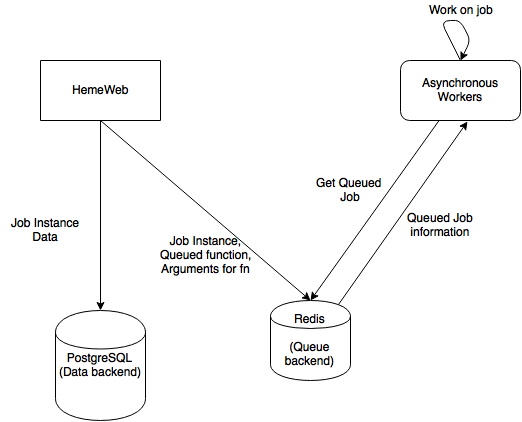
\includegraphics[keepaspectratio=true,scale=0.5]{../resources/images/hemeweb_master_components.png}
 }
\captionof{figure}{HemeWeb architecture}\label{fig:hemeweb-components}%      only if needed  
\end{minipage}

\vspace{1cm}

Figure \ref{fig:hemeweb-components} above illustrate how HemeWeb  application process interacts with the other components inside the master instance. It also illustrates how user's HTTP request start a chain of events inside the master master instance that will eventually return a response to the user's browser.

To start, user's browser will send an HTTP request to the master instance. This request will be captured by Nginx process that will act as a reverse proxy.  Nginx\footnote{\url{https://www.nginx.com}} will proxy the HTTP request towards the correct web application server process or serve static files depending on the requested URL. If the request is routed to the web application, HemeWeb web application which is handled by green unicorn\footnote{\url{http://gunicorn.org}} HTTP server will accept the request. This library will run the HemeWeb python code to process the HTTP request by the user. Depending on the type and path of the request, the web application will serve a static HTML as a response, or handle job-related logic that might interact with another part of the system. One of the components the web application might interact with is the PostgreSQL database\footnote{\url{https://www.postgresql.org}}. The database will persist job information locally on the instance to provide persistent information between HTTP request. However, it will be wiped out when the master instance is terminated and is not shared between HemeWeb instances.

Another part of the master instance the HemeWeb application can interact is with the queuing system. HemeWeb can submit a job into the queue which uses Redis datastore\footnote{\url{http://redis.io}} as the queue backend. HemeWeb uses third party library called Django-rq that handles asynchronous background tasks handling using Redis backend. It uses the pub / sub mechanism of Redis to create a lightweight background job workers. HemeWeb process will store the function to be executed, the job instance and parameters to used by the function into the Redis backend. A background worker will look at the queue at an interval and work on a job if there's any in the queue. The worker will execute the function and update the instance with relevant job execution result. Finally, the worker will go back to being idle waiting for next job to be executed.

\subsubsection{Docker components}

\vspace{1cm}

\noindent%
\begin{minipage}{\linewidth}% to keep image and caption on one page
\makebox[\linewidth]{
  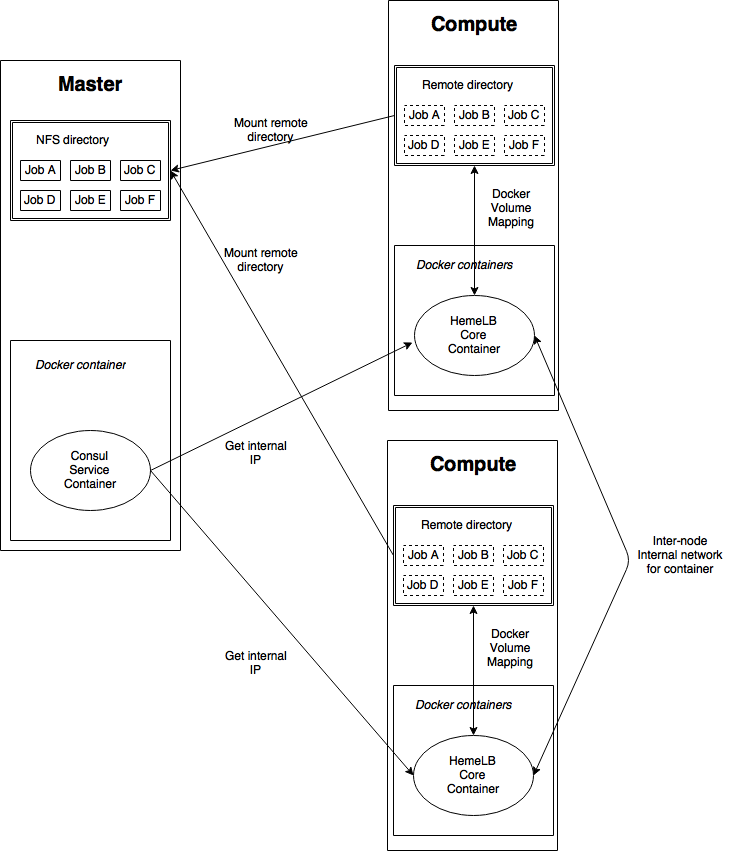
\includegraphics[keepaspectratio=true,scale=0.5]{../resources/images/hemeweb_docker.png}
 }
\captionof{figure}{HemeWeb Docker component}\label{fig:hemeweb-docker}%      only if needed  
\end{minipage}

\vspace{1cm}

In this section, I will discuss the interaction between Docker components and the hosts. As illustrated on figure \ref{fig:hemeweb-docker}, each host will run Docker service to run specific Docker container depending on their purpose.

In the master instance, a consul container is constantly running to provide inter-container communication mechanism. Consul\footnote{\url{https://www.consul.io}} is used by the Docker containers to coordinate the internal networking communication between them. In a host, multiple containers can be started without conflicting IP because they can communicate via the host. However, in HemeWeb the communication between containers will go beyond single hosts. Containers will need to communicate with other containers living on other hosts. Consul service is needed to coordinate this communication.

On the other hand, on the compute nodes, only HemeLB core container is run. The compute nodes will be started by a job submission to HemeWeb. After the nodes are started, HemeWeb process will instruct the compute nodes to pull the specified HemeLB core container version from Docker hub. If the specified version is locally cached on the compute nodes, no network activity will be made. HemeLB core container is then started to accept simulation command.

To start the simulation, the HemeLB core containers requires the job directories to be exported via Networked File System interface. HemeWeb process in the master node will prepare the job directories with the correct folder and files locally in the master node. Every job submission to HemeWeb will create a specific folder for storing submitted job-related files. The exported job directories will then be mounted by the compute nodes provisioned for the simulation. Finally, HemeLB simulation can use the mounted job directories to read input from and write output to.


\subsubsection{Job instance structure}

As mentioned above, HemeWeb uses Django web framework to handle web functionalities. Django framework follows the object-oriented principle where everything is modeled as an object. Job information that is handled by HemeWeb is also modeled as an object that is derived from object class of Django. Literally named \textbf{Job}, is a class that represents simulation information. Each instance of this class will contains information specific to a simulation instance. \textbf{Job} class inherits from \textit{django.db.models.Model} class that is included within Django framework. HemeWeb \textbf{Job} class extends this basic class and add functionalities specifically related to job information.


HemeWeb's Job class has the following attributes:
\begin{itemize}
    \item id:  This is a unique UUID field that represents the Job ID. UUID field was chosen because it is appropriate for the possibility of sharing the job simulation files between different deployment of HemeWeb. UUID can prevent clashes of job ID between these instances.
    \item input\_file, stl\_file, profile\_file, output\_file, configuration\_file:  These attributes keep track of the files that are used by the job. It is stored as the path to the file in the local filesystem, but with Django functionalities, HemeWeb can work with the file as an object.
    \item container\_image:  This attribute determines which container of HemeLB core will be used in the simulation. Currently, the choice of the field's value is set manually in the codebase. 
    \item instance\_type: This determines which compute node type will be started for the simulation. 
    \item instance\_count: This attribute determines how many compute node will be started for the simulation. Currently, this is also set manually in the source code. 
    \item status: The attribute to determine Job's status, whether it is \textit{queued, added, done, failed, etc}
    \item created: Attribute to keep track when the job is created
    \item updated: Attribute to keep track when the job is updated 
\end{itemize}



\subsubsection{Job directory structure}

Each simulation done with HemeWeb have its own job directory. These directories are located in the master instance and are shared with the compute node. To provide a clearer picture how the application package and work with the job's files, I will discuss how HemeWeb structure each job's files.


\begin{lstlisting}
<UPLOAD_FOLDER_DIR>/<JOB_ID>
<UPLOAD_FOLDER_DIR>/<JOB_ID>/inputs/*
<UPLOAD_FOLDER_DIR>/<JOB_ID>/logs/*
<UPLOAD_FOLDER_DIR>/<JOB_ID>/outputs/*
<UPLOAD_FOLDER_DIR>/<JOB_ID>/metadata
\end{lstlisting}

Listing above illustrates the structure of a job instance's directory structure.  The first component of all job instance's directory is the UPLOAD\_FOLDER\_DIR. This is the path to a directory in which HemeWeb will upload all files. To change this parameter, one should change the path in the HemeWeb settings file and restart the web application so the changes took place.

The next part of the directory structure is the job folder named with its ID. The ID will be generated by HemeWeb using Universally Unique Identifier (UUID) scheme. More specifically, UUID Version 4 that depends on the random number. Using UUID is important for HemeWeb because it is accurately approximated to have a really low chance of producing duplicate ID. Hence, HemeWeb does not have to take care of the possibility of jobs having duplicate ID.

Next, we have the inputs folder inside the job folder. This is where all the inputs and configurations are stored by the web application. There's also logs folder, where the job stdout, stderr, and HemeLB logs are stored. The web application will read from this folder and make it available on the web interface. Outputs folder will be used by the HemeLB simulation to write output files in this folder. One final file is the metadata file. This file is used by the web application to store the state of the job. The job is pickled into this metadata file so when it is downloaded, the web application can unpickle the state of the job instance and it is preserved, ready to be used for another simulation.

A Job instance is preserved with this job directory structure. This allows job information to be preserved in an external storage that can be used for backup. HemeWeb currently supports uploading job directory to amazon simple storage service (S3). However, backup is not the only purpose for this functionalities. By making job directory files available to the public, independent peers can download these files and run the simulation with correct files and configurations. It allows peers to replicate a simulation exactly or with modifications.

\subsection{Simulation workflow}

\vspace{1cm}

\noindent%
\begin{minipage}{\linewidth}% to keep image and caption on one page
\makebox[\linewidth]{
  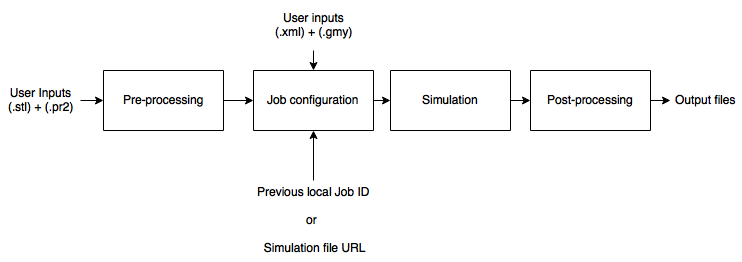
\includegraphics[keepaspectratio=true,scale=0.5]{../resources/images/implementation.png}
 }
\captionof{figure}{HemeWeb flow}\label{fig:hemeweb-implementation}%      only if needed  
\end{minipage}

\vspace{1cm}

Figure \ref{fig:hemeweb-implementation} illustrates how the HemeWeb web application works. HemeWeb currently consists of 4 core activities that will be discussed in details in the following section.

\subsubsection{Pre-processing}

In this step, HemeWeb handles pre-processing of inputs that are needed so that HemeLB simulation can parse the files. The user provides a geometry file (.stl) and a profile file (.pr2) to the web application for processing. HemeWeb will then create a job instance with these two files, save them locally on master instances and queue the pre-processing job.


\vspace{1cm}

\noindent%
\begin{minipage}{\linewidth}% to keep image and caption on one page
\makebox[\linewidth]{
  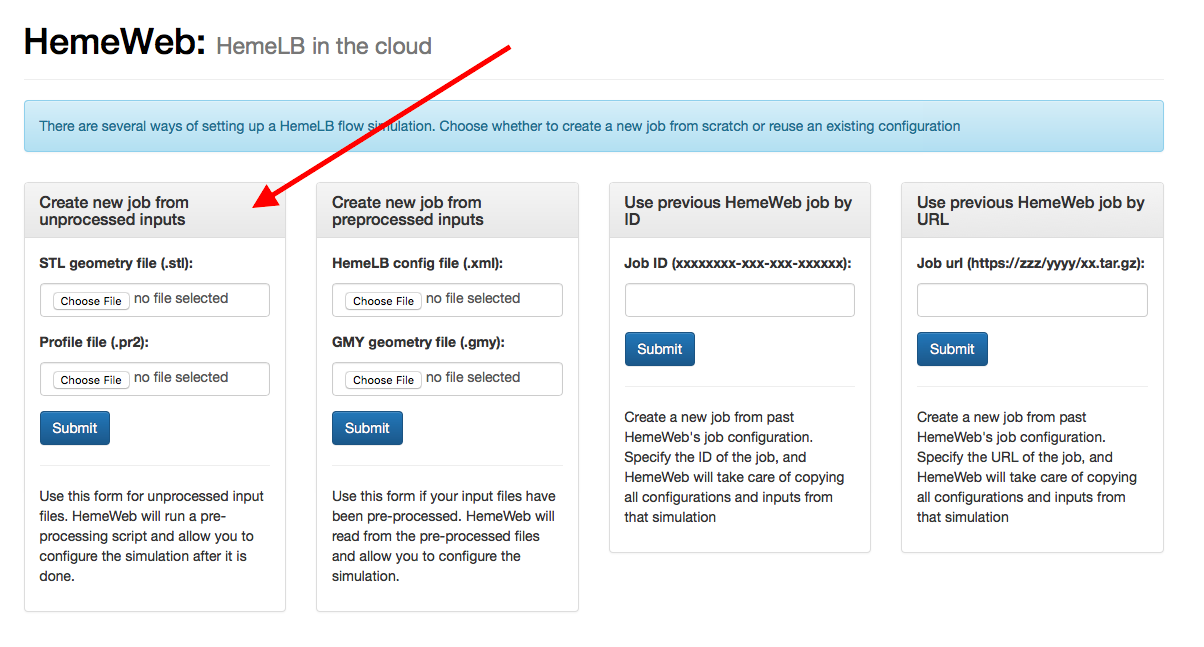
\includegraphics[keepaspectratio=true,scale=0.4]{../resources/images/pre-processing}
 }
\captionof{figure}{HemeWeb pre-processing form}\label{fig:hemeweb-pre-processing}%      only if needed  
\end{minipage}

\vspace{1cm}


Figure \ref{fig:hemeweb-pre-processing} shows HemeWeb user interface to upload the unprocessed files.  After submission of both files and job being queued, the asynchronous worker on the master instance will work on the job whenever they are free. It will run the pre-processing python script to generate the geometry files and HemeLB configuration file. These files will then be saved to the master instance, and HemeWeb will track these files by recording the path to these files on the job instance. Now the job instance is ready for the next step. of the workflow.

\subsubsection{Job configuration}

In this step, HemeWeb application will take a job instance with correctly set geometry file (.gmy) and HemeLB configuration (.xml). However, there are multiple ways that HemeWeb can get this correctly set job instance. As illustrated on Figure \ref{fig:hemeweb-implementation} , there are 4 possible entry points for this step. The web interface for these 4 entry points are also shown on Figure \ref{fig:hemeweb-pre-processing} They are:

\begin{itemize}
    \item \textbf{From the post-processing step.}
    	These files are generated from the previous pre-processing step. The job instance is directly used in this step
    
    \item \textbf{User's provided geometry and configuration file.}
    	User have pre-processed their own file locally, or have their own geometry and configuration files available. HemeWeb will create a new job instance, save both files and keep them tracked with the job instance.
	
    \item \textbf{User's provided previous job ID.}
    	There are two possible case when user specify previous job ID. First, the previous job is available locally on the HemeWeb instance. Second, the previous job is cached on the persistent storage on the cloud vendor and are not available locally. HemeWeb will download the previous file from the persistent storage if it is not available locally. It will then create a new job instance that copy the previous job's geometry file and configuration file to be used for further configuration.
    
    \item \textbf{User's provided simulation file URL.}
    	The last alternative is for user to provide the simulation file URL. Simulation files are uploaded to a persistent storage at the end of the workflow. These files, if made public, can be used by other instance of HemeWeb to download the simulation files and use it as a basis to create a new job instance. The way the system work is the same as using previous job ID, but its source is not its own persistent storage, but other people's simulation files.

\end{itemize}


After the job instance is created from one of the four way possible discussed above, HemeWeb will then ask users for the job configuration. 

\vspace{1cm}

\noindent%
\begin{minipage}{\linewidth}% to keep image and caption on one page
\makebox[\linewidth]{
  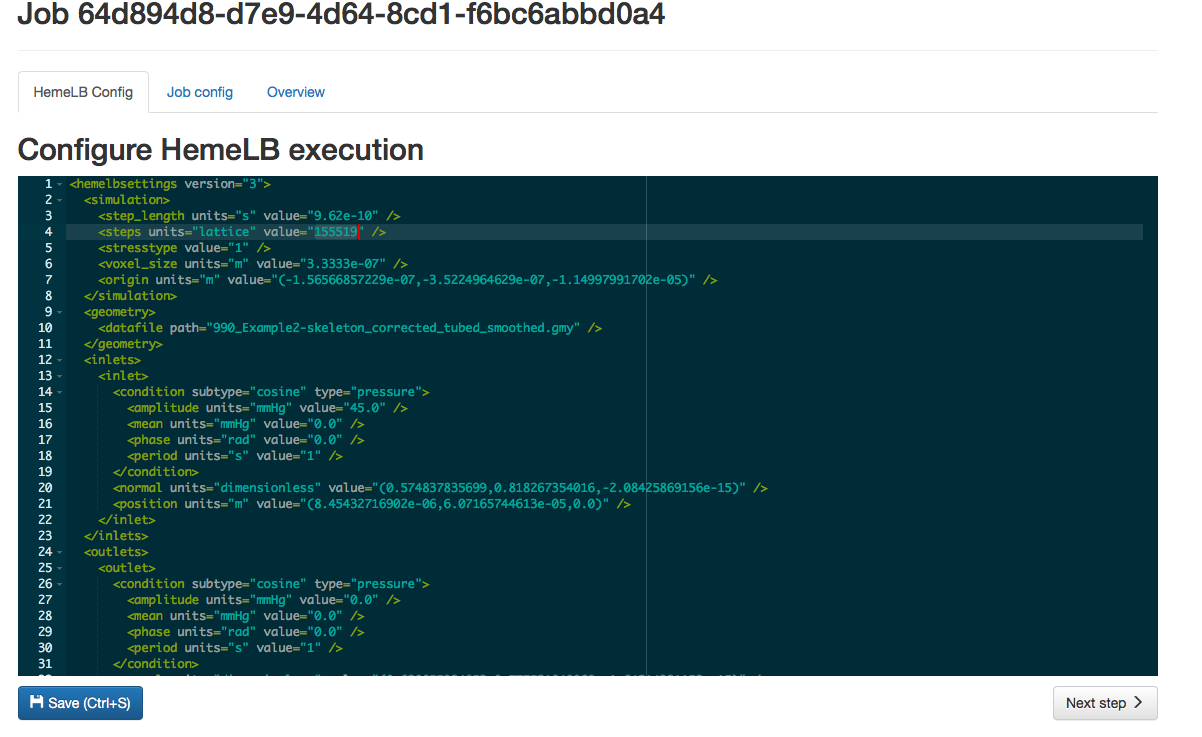
\includegraphics[keepaspectratio=true,scale=0.3]{../resources/images/configure1}
 }
\captionof{figure}{HemeWeb HemeLB configuration form}\label{fig:hemeweb-configure1}%      only if needed  
\end{minipage}

\vspace{1cm}

Figure \ref{fig:hemeweb-configure1} shows the interface where users are asked to configure the HemeLB simulation parameter. In this page, an online XML editor will be provided for the user to directly edit the .xml file that is provided by the users or from the  pre-processing step. Users can directly edit values that affect simulation execution like inlet pressure, outlet pressure, blood viscosity, and etc. After configuring the simulation parameter it will then be redirected to job configuration page.



\vspace{1cm}

\noindent%
\begin{minipage}{\linewidth}% to keep image and caption on one page
\makebox[\linewidth]{
  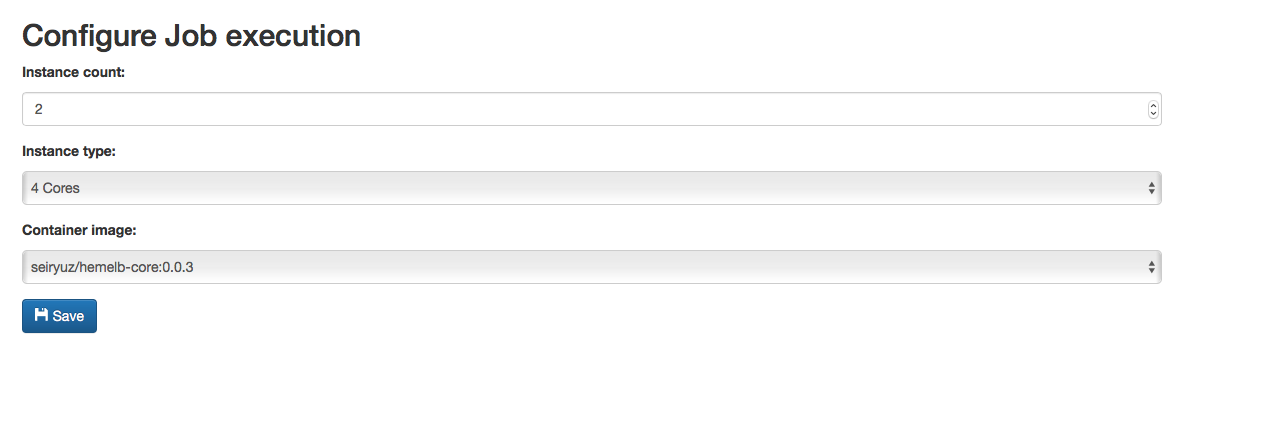
\includegraphics[keepaspectratio=true,scale=0.3]{../resources/images/configure2}
 }
\captionof{figure}{HemeWeb Job configuration form}\label{fig:hemeweb-configure2}%      only if needed  
\end{minipage}

\vspace{1cm}

Figure \ref{fig:hemeweb-configure2} shows the job configuration page. This page asks users about the parameter in which the simulation will be run with. These parameters are instance count, instance type, and HemeLB core container version. Instance count will determine how many compute node will be provisioned for this simulation by HemeWeb. Instance type will determine what type of compute node will be started, and the HemeLB core container version will determine what version of the container the compute node will use to run HemeLB simulation. After all of these parameters are set, users will be asked to confirm the job execution in the overview page. In the page, the user can then finally queue the job into the queue system.



\subsubsection{HemeLB simulation}

Once job instance is queued into the simulation queue, a free asynchronous worker will pop the queue and run the job. The worker will start up the configured amount and type of server instance from the cloud provider. These instances will then be further reconfigured by an ansible script so that it points to the correct master instance address. Next, input files are shared via Networked File System(NFS), the compute units will mount the input folders to their instance. 

The correct HemeLB core container version will be pulled from Docker hub in the next step. This step will skip the download if the container asked are already cached in the image for compute units which are prepared on the deployment part. After all of these are done, then the simulation can finally begin. Master node will issue an MPI command to be run by the leader of compute nodes. The leader of compute node then will run this MPI command in the Docker container. This command will be run on multiple compute node if it is configured as such in the previous steps. 

The HemeLB simulation will run until outputs are produced. The output will be written back to the correct output folder in the shared folder. This means that the master instance will have access to the outputs file and can do further processing. This step ends with the termination of the instances.

\vspace{1cm}

\noindent%
\begin{minipage}{\linewidth}% to keep image and caption on one page
\makebox[\linewidth]{
  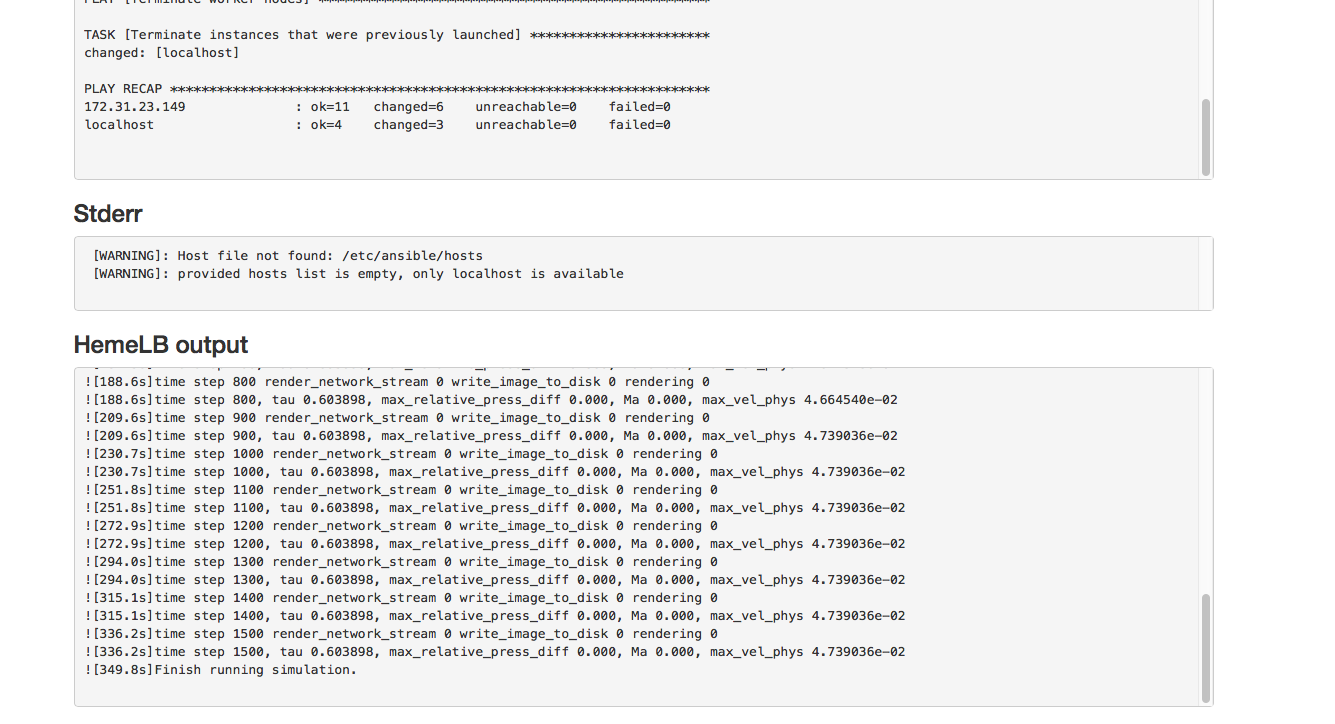
\includegraphics[keepaspectratio=true,scale=0.3]{../resources/images/output}
 }
\captionof{figure}{HemeWeb Job logs}\label{fig:hemeweb-output}%      only if needed  
\end{minipage}

\vspace{1cm}

Figure \ref{fig:hemeweb-output} shows how the Job execution will produce logs that can be viewed on HemeWeb web application. During simulation, logs are written to the respective job folder and are served to the browser by the HemeWeb app. Showing the logs allows users to easily view the progress of the job or even debug failed job.


\subsubsection{Post-processing}

After HemeLB simulation is finished, HemeWeb web app will do some post-processing steps to make sure the output files can be viewed easily. The outputs from HemeLB simulation are structured in such a way that makes it efficient to write in parallel. However, these outputs cannot be viewed by visualization system like Paraview. What HemeWeb will do is to pipe the output files to two python scripts that will format the output into a format that can be understood by ParaView.


However, the post-processing steps are not done yet. There are further steps that HemeWeb took to make sure that the simulation files, configurations, and results are preserved externally. HemeWeb will package the job directory, compressed it, and upload it into persistent storage that cloud vendors provide. As the time of writing, HemeWeb only supports amazon simple storage service. The simulation files are uploaded to this storage and made accessible to the public so other HemeWeb instance can use them. Also, with the job files persisted on persistent storage, the next HemeWeb instance deployed can take advantage of these files that it can use it as previous jobs to be used on current deployment





\subsection{Implementation Challenge}


In this section, I will try to outline and discuss the challenges in implementing this project, and if any, the solution that I choose.

\subsubsection{Cloud vendors features and API difference}

The challenge in developing the deployment script is the difference of cloud vendors' API and features.  This has led to some problems when trying to create a common API to do a certain task. One notable problem is that the absence of image creation from running instance feature from one of the cloud vendors. Image creation feature is not an essential requirement of the project. However, with an image creation, the compute nodes that will be requested by the web application can be configured much quicker because all the pre-configuration that are done during the deployment phase. However, one of the cloud vendors does not have this feature. This creates a situation where there is no elegant way to create image with the deployment script and users are asked to manually created the image on the web interface

\vspace{1cm}

\noindent%
\begin{minipage}{\linewidth}% to keep image and caption on one page
\makebox[\linewidth]{
  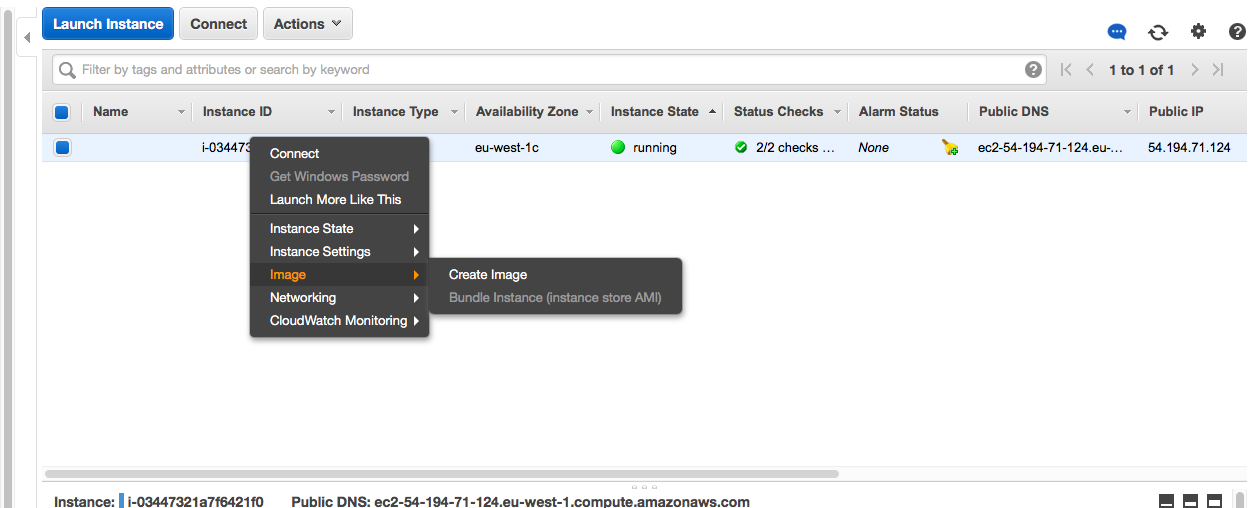
\includegraphics[keepaspectratio=true,scale=0.4]{../resources/images/hemeweb-challenge-1.png}
 }
\captionof{figure}{Manual image creation instead of automatic}\label{fig:hemeweb-challenge-1}%      only if needed  
\end{minipage}

\vspace{1cm}

Figure \ref{fig:hemeweb-challenge-1} shows how users are instructed to manually create an image from running instance. Users have to go the web interface of specific cloud vendors, right-click on the running instance, and create the image from it. This is a simple workaround which is less complicated compared to accommodating different or missing features and API from different cloud vendors.


Another problem is the time constraint. Due to the time constraint, I cannot achieve full compatibility with all cloud vendors. The development time is mainly focused on amazon web service because it has all the features HemeWeb need. However, this means that the codebase is currently tied to one cloud vendors. Features like automatically reading past simulation files from cloud storage and uploading simulation files are tied to amazon infrastructure. It is possible to refactor these functionalities out to become more generic, however for the interest of time, I decided not to.

\subsubsection{Security}

Another challenge that I face during the development of HemeWeb is to handle the security of the application. However, security is not the main focus of this work and is apparent in the development of the application. I will still discuss the security issues so that I can give an objective assessment of the application.

The first security issues that I found is with regards to the compute node security in some cloud vendors. Digital ocean, for example, does not provide a "real" private networking option within compute nodes. They have a "shared" private networking options that allow other compute nodes, which are not even on your account have network connectivity to your node. Theoretically, this allow other people access to your private compute node if they have the credentials. In this case, I made sure that all the compute nodes have a sensible access policy to deter unauthorized access to the nodes. I only allow ssh with a public key and disabled password access to ssh. Also, it is also much better to choose cloud vendors that have real private networking like AWS. In which, the compute nodes are not accessible to other nodes that are not part of your own private network. This is much more secure and sensible.


Another security issue is on how compute and master node share simulation job's files. It currently uses Network File System without any security measures towards the nodes that try to mount it via the private network. There is an opportunity to secure this communication by encrypting the job files, but it is not currently done.


\section{Development process}

The development process is divided into 5 phases. The planned phases are as follow:

\begin{enumerate}
    \item{Separate HemeLB core into its own container}
    \item{Orchestrate the deployment of HemeLB cluster / infrastructure}
    \item{Develop HemeWeb to accept user input}
    \item{Extends HemeWeb to handle geometry generation workflow}
    \item{Extends HemeWeb to handle domain definition step or Viewing of HemeLB simulation result}
\end{enumerate}

The development process loosely follows the agile method in which I regularly meet with the stakeholders every week to give an update and gather feedback on the project. The phases are designed in such a way to minimize the risk of having nothing at all during the end of the project phase. This is due to that HemeWeb can work on its own after finishing step 3. The HemeLB simulation can be done on its own. The rest of the steps are there to extend the functionalities of the HemeWeb to cover more functionalities.

During the first week of the development, I focused more on stripping the HemeLB core container into its own. I researched on how Docker and Dockerfile work, and finding out what are the issues with the current container. After identifying the issues, which are ssh service and full of functionalities which are not essential, I stripped down the image and changed the base image so that the container could avoid the mentioned problems. I end up with smaller container size and it is available online on https://hub.docker.com.

However, one particular issue with what I have currently is that the Dockerfile is published as a part of the HemeWeb source code. It should be tied down to the HemeLB development instead of HemeWeb. Currently, the development model of HemeLB is that there is an internal private repository where the less than stable build is pushed to it, and there are public repositories where only stable builds are pushed into. The release process should include adding the Dockerfile towards the core HemeLB source code repository and tagging the release correctly. HemeLB core containers should then be built automatically on Docker hub with regards to additional tags being pushed to the public repository.


After the development of HemeLB core container, I then focused on how the architecture could be primed for the HemeLB simulation. It involves on configuring the servers and all supporting infrastructures on cloud vendors to be ready for HemeLB simulation. Network configuration, security configuration, Docker configuration, and other should be handled automatically. I elect to choose ansible orchestration software because it is closely related to python language that I used. 

In this phase, I successfully achieve the provision and deployment process that with the correct credentials and authorization, the script could provision and configure the architecture correctly so it is ready for HemeLB simulation. In addition to that, I successfully created the script so that it will be cloud vendors agnostic. I can deploy the architecture to google cloud vendors, amazon web service, and digital ocean.

However, it is to be noted that the deployment process that I achieve can only run HemeLB simulation from the command line. I have not considered the web application installation and configuration at this point of the deployment. I only considered the infrastructure being built and configured for HemeLB simulation.


Next, I started developing HemeWeb web application. I choose Django web application framework due to my experience with it. I created a basic interface, where job simulation is listed on the index page on the home interface. After that, I added a basic interface to add new job with a geometry file and HemeLB configuration file. The web application will then add those input files into a newly created job instance and configure the job instance in the job configuration step. The job will then be submitted. 

Here I developed a separate ansible script that will be called when a queued job is being worked at. The ansible script is responsible for starting up compute nodes needed by the job and executing HemeLB simulation. After the simulation is done, the script is also responsible for correctly terminating the compute node.

After the basic HemeWeb web application is achieved, I extend it to handle pre-processing. I added an extra form in the adding new job form to handle a profile file and geometry file. These two files will be converted into a geometry file and HemeLb configuration file that the job configuration steps expect. In addition to adding the interface, I also added a new function on the job instance that will run this pre-processing step on the background. 

Lastly, due to the limited time, I can only manage to run a small post-processing step on HemeWeb. What I did was adding post-processing step that converts the Extracted results from HemeLB output into a format that can be viewed by third party software, ParaView. The results are piped into two scripts that will output a .vtu that is compatible with ParaView. This is done during the background activity after simulation result is outputted. However, currently, this is done on the master node.

In addition to that, I also managed to add persistence capability to HemeWeb application. What I did was to package the job simulation folder into a compressed archive and upload it to persistent storage service of cloud vendors. These archives can be queried by another instance of HemeWeb to get previous job IDs available for the particular cloud vendor account used to deploy HemeWeb.  Also, the job simulation file URL is also showed on the web interface. Making it easy for the users to share the simulation file with their peers.





% Activate the following line by filling in the right side. If for example the name of the root file is Main.tex, write
% "...root = Main.tex" if the chapter file is in the same directory, and "...root = ../Main.tex" if the chapter is in a subdirectory.
 
%!TEX root =  dissertation.tex

\chapter[Evaluation]{Evaluation}
In this chapter, I will discuss on the system's evaluation. Success will be measured by answering these questions:

\begin{itemize}
    \item Can users run a simulation using our system ?
    \item Can users reproduce past simulations using our system ?
    \item Are users satisfied in using our system ?
    \item Are users more likely to run a simulation using our system compared to the command line ?
    \item How does it perform compared to the existing infrastructure ?
\end{itemize}


In answering questions above, I conduct two sets of evaluation. First, an online questionnaire was conducted to measure user's experience and system's usability. And secondly, a performance analysis comparing the performance of HemeLB between dedicated hardware against cloud vendors. The questionnaire will answer most of the questions related to user experience and usability above, while the performance benchmark will be the basis for performance evaluation and justification in using HemeWeb.

%These questions will be answered in two different evaluations. First, an online questionnaire was sent to the target audience of HemeWeb. In the questionnaire, testers will be asked to run two scenarios and answer questions to measure their experience. These answers will be the basis for answering most of the questions above. In addition to the questionnaire, I will measure the performance of HemeWeb in running HemeLB simulation by running benchmarks and comparing the raw performance number. These benchmarks will be the basis of the performance measure of the evaluation.

\section{Questionnaire}

In measuring user's experience, I created a questionnaire for HemeWeb using google form. The questionnaire was live for a week, from 3rd of August 2016 until 10th of August 2016.

%I created a questionnaire that will measure user's experience in using HemeWeb. This questionnaire was created and shared using google forms. It ran online for 10 days from 1st August 2016 - 10th August 2016.

At the start of the questionnaire, respondents are asked about their background information. This information will be used to provide demographic insight on the respondents and how it affect the type of answers the respondents will most likely give. Respondents will be asked to fill out their age, gender, job, discipline, and level of familiarity with various software tools. From their responses, I can determine whether the sample population is representative of the target audience.

%In the questionnaire, testers are asked to answer about their background information to provide demographic insight on them. Testers are asked to fill in their background information like age, gender, job, discipline. In addition, this part also ask about testers' familiarity with browsers, installing software from source code, and computational fluid dynamic software. These are required for us to determine whether our sample population is representative of the target audience of the application developed.

The questionnaire is set to make tester run specific scenarios that HemeWeb is developed for. These scenarios are running a simulation using the web interface and reproducing past simulation with it. Testers running the scenario are given an option to skip the scenario and go straight to the questions below it to measure their experience if they find it too difficult. 

The first scenario asks testers to run a simulation with given inputs. The questionnaires list two input files, a geometry file and a HemeLB configuration file that testers will need to download to their computers. After downloading the input files, testers are asked to open their browser and go to a specific URL where HemeWeb was deployed for the evaluation purposes. In that URL, testers will then add a new simulation job with the downloaded files, configure the job, and submit the job to the queue. The scenario ends when the job is submitted.

The second scenario asks testers to reproduce past simulation with a given URL that contains past simulation files. It asks testers to create a new job from the given URL instead of using files that are downloaded in the past scenario. After creating a new job, testers then will change some configuration and parameters from the past scenario and submit the job. The scenario also ends when the job is submitted.

Following each scenario are questions to measure whether users skip the scenario and an after-scenario questionnaires that users have to answer. The after-scenario questionnaire is based on the usability measurement at IBM developed by James R Lewis \citep{lewis1995ibm}.  It measures users' usability satisfaction with the system with regards to given scenario. The questionnaire give 3 statements which testers should agree or disagree, they are:

\begin{itemize}
	\item Overall, I am satisfied with the ease of completing the tasks in this scenario
	\item Overall, I am satisfied with the amount of time it took to complete the tasks in this scenario
	\item Overall, I am satisfied with the support information (online-line help, messages, documentation) when completing the tasks
%	\item If any, give suggestions on what could be better
\end{itemize}

In addition to above questions, there are some questions about the tester's willingness to do exactly the same tasks as the scenario, but with the command line. This question will measure user's willingness in using the command line interface compared to the web interface. 


After running both scenarios, testers are then redirected to the final questionnaire. The Post Study System Usability Questionnaire which is based on the same work by James R Lewis \citep{lewis1995ibm}. In this questionnaire, testers are given 19 statements where they should agree or disagree, they are:
\begin{itemize}
	\item Overall, I am satisfied with how easy it is to use this system
	\item It was simple to use this system
	\item I can effectively complete my work using this system 
	\item I am able to complete my work quickly using this system
	\item I am able to efficiently complete my work using this system
	\item I feel comfortable using this system
	\item It was easy to learn to use this system
	\item I believe I became productive quickly using this system
	\item The system gives error messages that clearly tell me how to fix problems
	\item Whenever I make a mistake using the system, I recover easily and quickly
	\item The information (such as online help, on-screen messages, and other documentation) provided with this system is clear
	\item It is easy to find the information I needed
	\item The information provided for the system is easy to understand
	\item The information is effective in helping me complete the tasks and scenarios 
	\item The organization of information on the system screens is clear
	\item The interface of this system is pleasant
	\item I like using the interface of this system
	\item This system has all the functions and capabilities I expect it to have 
	\item Overall, I am satisfied with this system
\end{itemize}

In addition to the above questions, testers also will be asked to list the most negative aspects and positive aspects of the system if they have any. These questions will measure users satisfaction with the overall system, whether it is useful, whether the information given by the system is any good, and the interface quality.

%There are 4 sections of the questionnaires. The first one is to capture the demographic of the testers. Testers are asked to fill in their background information like age, gender, job, discipline. In addition, this part also ask about testers' familiarity with browser, installing software from source code, and computational fluid dynamic software.

\section{Performance benchmarks}

The second part of the evaluation is the performance benchmark. HemeWeb is running HemeLB simulation outside its original scope of being used on a highly parallel computing resources like a supercomputer. This could have an interesting impact on the performance of the system because cloud vendors, being much more easily accessible and provisioned, have an underlying infrastructure difference with the stand-alone infrastructure. This performance benchmarks will then measure whether the impact on the performance justify the claimed usability benefit that we measure on the first half of the evaluation.

The performance benchmark will be done by the internal tooling that is baked inside HemeLB. Every HemeLB simulation will produce a report file that measures the performance of said simulation. On this evaluation, I will compare the performance of HemeLB simulation on four different scenarios to measure the performance impact on having HemeLB simulation on the cloud with Docker containers. They are:
\begin{itemize}
	\item{ARCHER supercomputer}
	\item{INDY2 HPC Cluster}
	\item{Cloud computing infrastructure with AWS EC2}
\end{itemize}

The benchmark on ARCHER supercomputer will be the gold standard of the performance. It's a gold standard because the infrastructure has a clear purpose of being used for the HPC application. It has the necessary resources and components that are tailored for it. It should be the ideal performance scenario. Next, the local computing infrastructure. This paints a picture if how HemeLB will perform on a private local infrastructure which is built to run highly parallel jobs. This will be the measure that can be used if HemeLB is to run on private infrastructure.

The last benchmark will be done to measure the performance of HemeLB simulation compared to the local infrastructure. Cloud computing vendors have an underlying difference with regards towards how the infrastructures are structured and connected together. This could have an inherent performance different with a standalone infrastructure. This benchmark will measure this difference.

% Activate the following line by filling in the right side. If for example the name of the root file is Main.tex, write
% "...root = Main.tex" if the chapter file is in the same directory, and "...root = ../Main.tex" if the chapter is in a subdirectory.
 
%!TEX root =  dissertation.tex

\chapter[Analysis]{Analysis}

\section{Usability result and analysis}

In evaluating HemeWeb's usability and capability to run and reproduce simulation, I conducted a usability evaluation via an online survey hosted by Google Form\footnote{\url{https://goo.gl/forms/toYsRwnGIGumMBUD2}}. Respondents are given 2 tasks to complete, which are to run a simulation and reproduce past simulation. After the tasks, they are given statements to respond to. Based on the answers, I analyze respondent's answers with regards to HemeWeb's usability.


\subsection{Demography}


\vspace{0.5cm}

\noindent%
\begin{minipage}{\linewidth}% to keep image and caption on one page
\makebox[\linewidth]{
  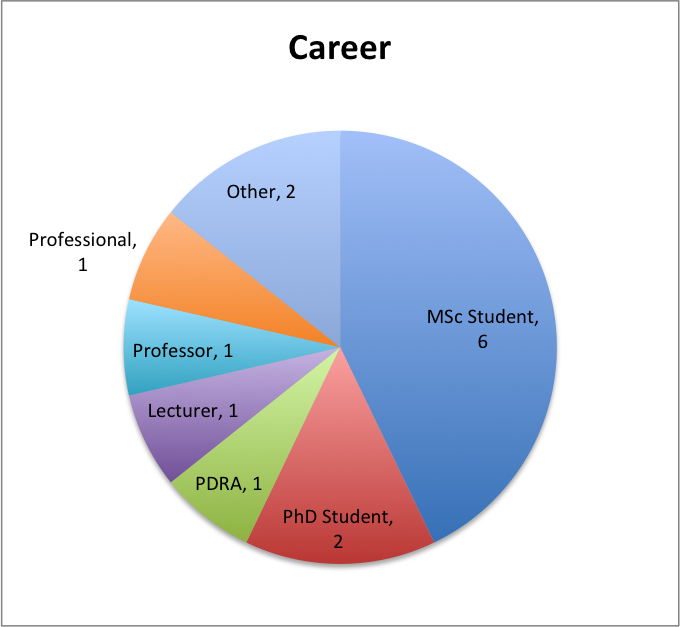
\includegraphics[keepaspectratio=true,scale=0.7]{../resources/evaluation/usability/career.png}
 }
\captionof{figure}{Career stage distribution} \label{fig:survey-career}%      only if needed  
\end{minipage}

\vspace{0.5cm}

\vspace{0.5cm}

\noindent%
\begin{minipage}{\linewidth}% to keep image and caption on one page
\makebox[\linewidth]{
  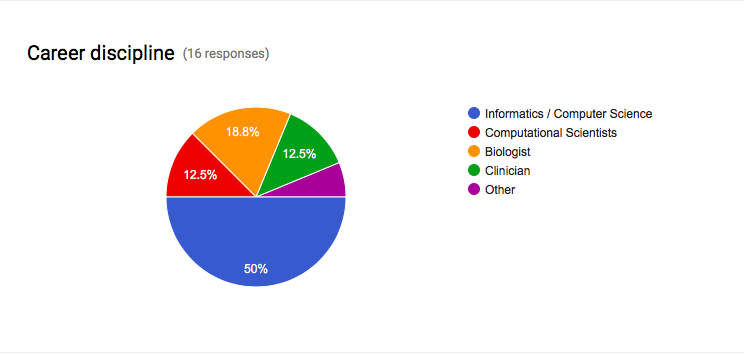
\includegraphics[keepaspectratio=true,scale=0.8]{../resources/evaluation/usability/discipline.png}
 }
\captionof{figure}{Career discipline} \label{fig:survey-discipline}%      only if needed  
\end{minipage}

\vspace{0.5cm}


The survey was filled by 16 respondents over the period of 10 days (3rd August 2016 - 10th August 2016)\footnote{Raw and compiled responses can be found at \url{https://github.com/SeiryuZ/HemeWeb/tree/master/documents/resources/evaluation/usability} \label{footnote:response}}. From all the responses, one of the respondent were unable to run both of the tasks, citing errors preventing him to run the scenarios which we cannot reproduce. Due to this problem, we have to remove this particular response from our analysis because it will not add meaningful information about the usability of the system when the scenarios are not run. In total, we got 15 valid responses out of the questionnaire period.

Figure \ref{fig:survey-career} and \ref{fig:survey-discipline} illustrates the distribution of career stage and discipline of our participants. Based on this distribution, we can further analyze the response we get on the survey questions based on their background. One meaningful comparison we can make is when we classify respondents based on their informatics-related discipline. 10 of our respondents, or 2 out of 3, are related to informatics background, while 5 of the respondents can be considered as domain experts which consists of Biologist, Clinician, and Biophysicist.


\vspace{0.5cm}

\noindent%
\begin{minipage}{\linewidth}% to keep image and caption on one page
\makebox[\linewidth]{
  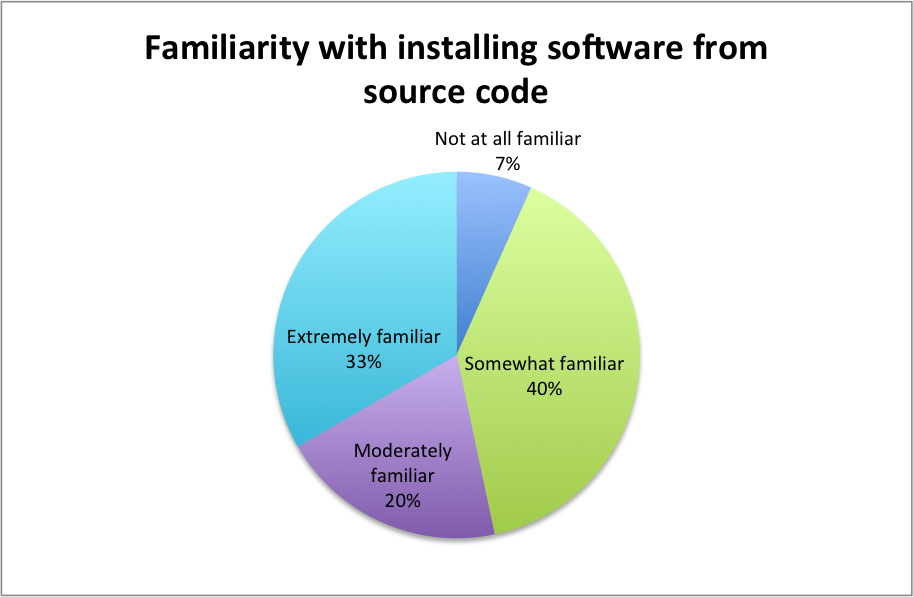
\includegraphics[keepaspectratio=true,scale=0.8]{../resources/evaluation/usability/source_code.png}
 }
\captionof{figure}{Familiarity with installing software from source code} \label{fig:survey-source}%      only if needed  
\end{minipage}

\vspace{0.5cm}

\noindent%
\begin{minipage}{\linewidth}% to keep image and caption on one page
\makebox[\linewidth]{
  
\includegraphics[keepaspectratio=true,scale=0.8]{../resources/evaluation/usability/browser.png}
 }
\captionof{figure}{Familiarity with web browser} \label{fig:survey-browser}%      only if needed  
\end{minipage}

\vspace{0.5cm}

\noindent%
\begin{minipage}{\linewidth}% to keep image and caption on one page
\makebox[\linewidth]{
  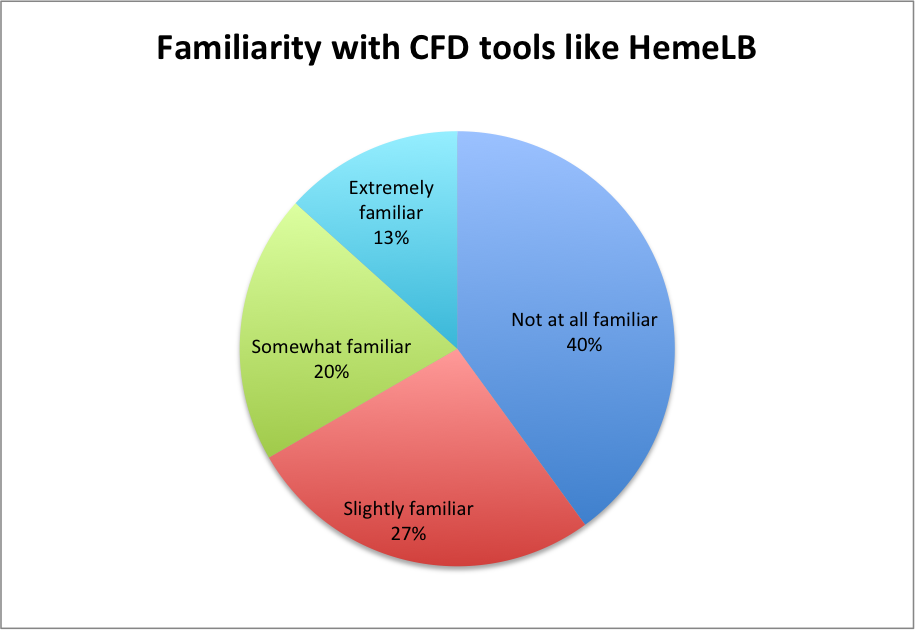
\includegraphics[keepaspectratio=true,scale=0.8]{../resources/evaluation/usability/hemelb.png}
 }
\captionof{figure}{Familiarity with CFD tools like HemeLB} \label{fig:survey-hemelb}%      only if needed  
\end{minipage}

\vspace{0.5cm}


We can also further classify analyze the respondents' response based on the familiarity with browsers, computational fluid dynamic tools, and installing software from source code. All of this are shown in Figure \ref{fig:survey-source}, \ref{fig:survey-browser}, and \ref{fig:survey-hemelb}.



\subsection{Scenario 1: Run a HemeLB simulation}

In this scenario, respondents are provided with two input files necessary for running a simulation. Respondents are asked to download the files beforehand and follow the instructions provided in the online questionnaire to run a HemeLB simulation using HemeWeb.  After running the simulation, Respondents are then asked to state agreement with three positive statements about HemeWeb that will measure their satisfaction with HemeWeb in running a HemeLB simulation scenario. 



\vspace{0.5cm}

\noindent%
\begin{minipage}{\linewidth}% to keep image and caption on one page
\makebox[\linewidth]{
  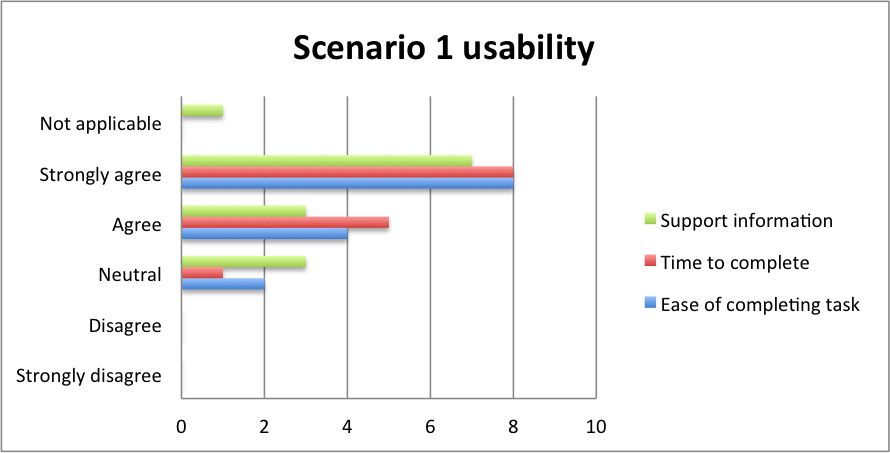
\includegraphics[keepaspectratio=true,scale=0.9]{../resources/evaluation/usability/scenario1_usability.png}
 }
\captionof{figure}{Scenario 1 usability} \label{fig:survey-s1-usability}%      only if needed  
\end{minipage}
\vspace{0.5cm}


Figure \ref{fig:survey-s1-usability} show the responses for the three positive statements about HemeWeb. From the 15 valid responses we get, all of them did not skip the instructions to run the simulation. From the responses, respondents tend to agree that they are satisfied with HemeWeb in running a HemeLB simulation. Respondents tend to equally agree on the three positive statements about the ease of completing a task, time to complete, and supporting information available to help complete the task. However, one respondent fills out "Not Applicable" towards the statement about HemeWeb giving them enough support information. This could mean that the scenario undertook to give enough information to agree or disagree with the statements.

In addition to the general sentiment of the respondents, we can also put a number value to the responses to further measure the satisfaction objectively. We can calculate the After Scenario Questionnaire(ASQ) score. To do this, we assign an integer value for each response; 1 for "Strongly disagree", 2 for "Disagree", 3 for "Neutral", 4 for "Agree", and 5 for "Strongly agree". With this value, we can take the mean of the response for each question as a single ASQ score for the respondent. If a respondent skips a question, we can take the average of the remaining responses as the score. With this mechanism, we can determine the respondent's average ASQ score, which is 4.36. This score falls between "Agree" and "Strongly agree", therefore, we can conclude that in general respondents tend to agree that they are satisfied with HemeWeb with regards to running a HemeLB simulation.



%Our hypothesis is that users will generally find using web interface is usable and the data seemed to support that. It is much easier for user to complete a task when using point and click interface rather than requiring them to recall commands to do the tasks, especially when they are not familiar with the tools.
%
%
%Next, respondents are given a high overview of replicating the tasks done in HemeWeb but using command line interface. Respondents are not asked to run the scenario in their command line interface because we cannot make sure the necessary tools are installed on respondent's computer.

\vspace{0.5cm}

\noindent%
\begin{minipage}{\linewidth}% to keep image and caption on one page
\makebox[\linewidth]{
  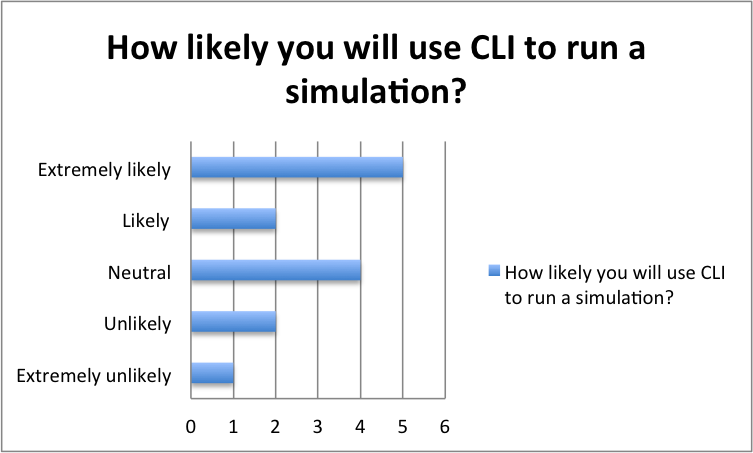
\includegraphics[keepaspectratio=true,scale=0.9]{../resources/evaluation/usability/scenario1_cli.png}
 }
\captionof{figure}{Scenario 1 command line preference} \label{fig:survey-s1-cli}%      only if needed  
\end{minipage}

\vspace{0.5cm}

\noindent%
\begin{minipage}{\linewidth}% to keep image and caption on one page
\makebox[\linewidth]{
  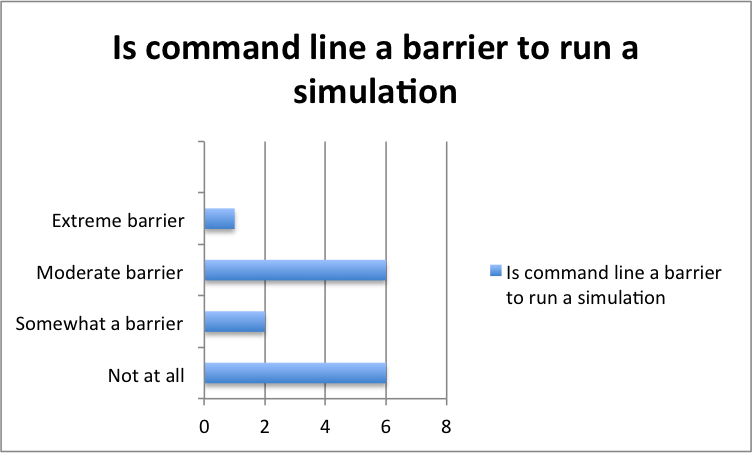
\includegraphics[keepaspectratio=true,scale=0.9]{../resources/evaluation/usability/scenario1_cli_barrier.png}
 }
\captionof{figure}{Scenario 1 barrier in using command line} \label{fig:survey-s1-cli-barrier}%      only if needed  
\end{minipage}

\vspace{0.5cm}

After the above sentiments about using HemeWeb to run a HemeLB simulation, respondents were asked about their sentiment about using command line interface(CLI) to do the same activity. Figure \ref{fig:survey-s1-cli} and \ref{fig:survey-s1-cli-barrier} shows the respondent's inclination in using CLI. Respondents are generally open to the likelihood of them running a simulation using CLI. If we quantify the results like we did with the ASQ score, we get 3.46, which is somewhere between neutral and likely. 

The distribution of the responses also is quite spread out, that respondents fill out all possible responses with   the highest frequency being "Extremely Likely" with 5 responses. However, we have to keep it mind the general background of the respondents that may explain the highest frequency answer being "Extremely Likely", which is about familiarity with installing software with source code. To build software with source code, one will interact with the command line interface quite often. 14 of our respondents answered at least somewhat familiar with building software from source code, that can explain that our respondents are mostly quite competent in operating command line interface and would not shy away in using the command line interface. In addition to that, 2 out of 3 respondents has backgrounds in informatics and computational science. This could in effect explains why the respondents feel they are likely and extremely likely to do the same in CLI. 

However, not all respondents who are at least somewhat familiar with building software from source code skew towards to the likely side of using CLI. There are respondents that, while familiar with the interface, running a HemeLB simulation using CLI is unlikely to be done by them. These responses might be explained by respondents' sentiment in using command line interface. This is further supported by the response of CLI being a barrier for the respondents. While 6 of the respondents think it is not a barrier at all to use CLI, 9 of the respondents answered at least it is somewhat a barrier. With 6 of the 9 respondents, feel it is a moderate barrier, and 1 of the 9 feel it as an Extreme barrier. From these results, we can safely say that using command line interface is a form of a barrier to run HemeLB for almost two-third of the respondents.





\subsection{Scenario 2: Reproduce past simulation}

In the second scenario, respondents are asked to reproduce past simulation with HemeWeb. They are given instructions in the online questionnaire to create a HemeLB simulation job from past simulation. They have to enter a URL that contains past simulation job and modifies the simulation parameters to avoid only replicating the past simulation without changes. After reproducing past simulation, respondents are then asked to state agreement with the same questions like they had in the first scenario. These questions will also measure their satisfaction with HemeLB in reproducing past simulation.


\vspace{0.5cm}

\noindent%
\begin{minipage}{\linewidth}% to keep image and caption on one page
\makebox[\linewidth]{
  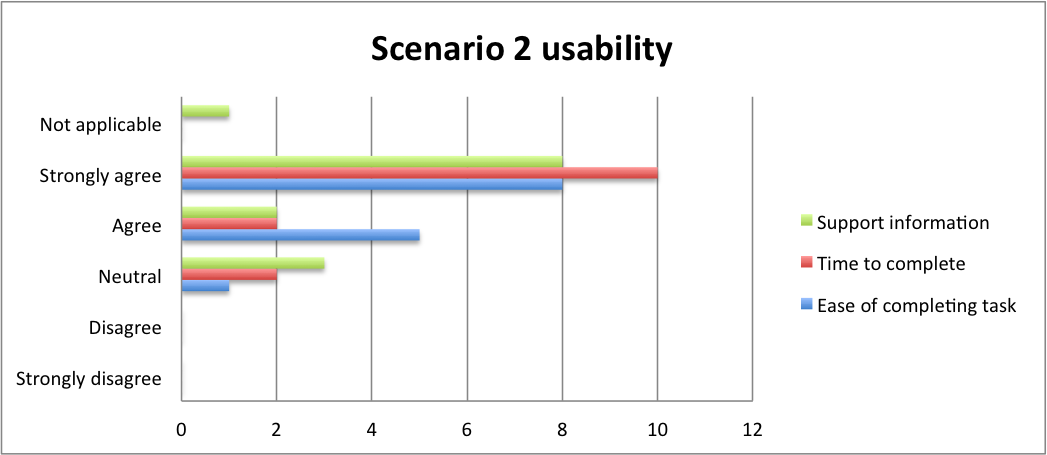
\includegraphics[keepaspectratio=true,scale=0.9]{../resources/evaluation/usability/scenario2_usability.png}
 }
\captionof{figure}{Scenario 2 usability} \label{fig:survey-s2-usability}%      only if needed  
\end{minipage}
\vspace{0.5cm}

Figure \ref{fig:survey-s2-usability} shows the general sentiment to the three statements that we provided. Generally, the response tends to skew towards agreeing that respondents are satisfied with HemeWeb with regards to reproducing past simulation. However, it has to be noted that 1 of the respondent skipped the instructions. This particular respondent did not give out any comments about encountering any problems, so we cannot deduce whether his skipping the instruction is due to usability problems or he just wants to skip it. Without further information, we cannot deduce why he skips the instructions.

Also, similar to the first scenario, one respondent fills out "Not Applicable" to support information statement. Once again, this could mean that the scenario does not provide the respondent with enough information to fill out their agreement to the statement. In a nutshell, respondents tend to agree that HemeWeb is satisfying to use for the purpose of reproducing past simulation. If we convert the responses to a numerical value, we will get 4.31 of ASQ score. Which is in line with the sentiment that I described. The ASQ score falls between agreeing and strongly agree towards the positive statements we provided.


\vspace{0.5cm}

\noindent%
\begin{minipage}{\linewidth}% to keep image and caption on one page
\makebox[\linewidth]{
  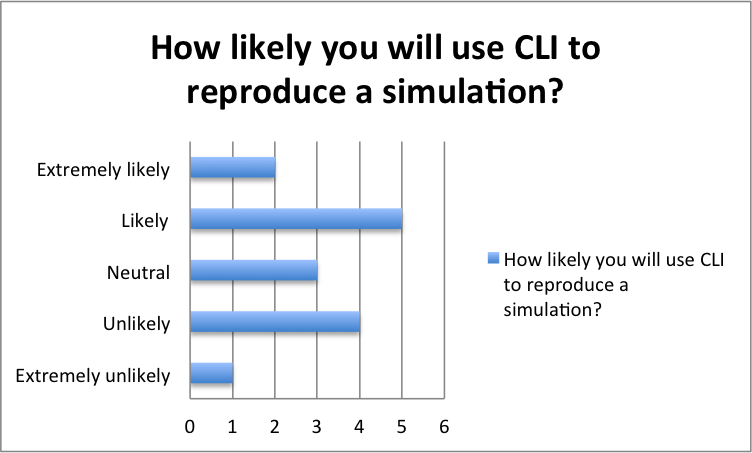
\includegraphics[keepaspectratio=true,scale=0.9]{../resources/evaluation/usability/scenario2_cli.png}
 }
\captionof{figure}{Scenario 2 command line preference} \label{fig:survey-s2-cli}%      only if needed  
\end{minipage}

\vspace{0.5cm}

\noindent%
\begin{minipage}{\linewidth}% to keep image and caption on one page
\makebox[\linewidth]{
  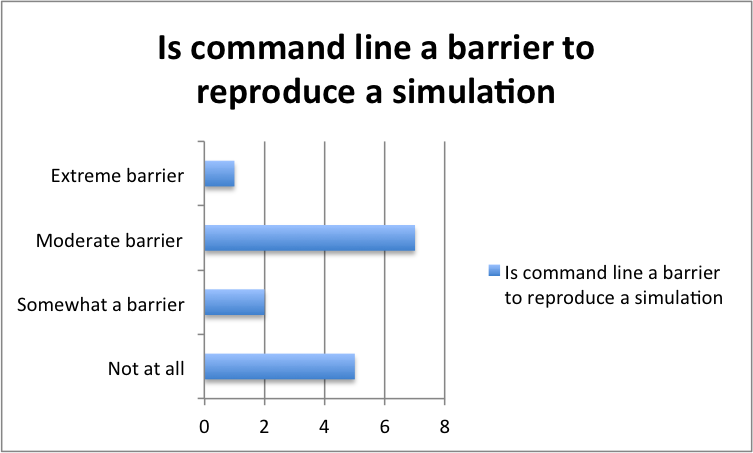
\includegraphics[keepaspectratio=true,scale=0.9]{../resources/evaluation/usability/scenario2_cli_barrier.png}
 }
\captionof{figure}{Scenario 2 barrier in using command line} \label{fig:survey-s2-cli-barrier}%      only if needed  
\end{minipage}

\vspace{0.5cm}

Respondents are then given high-level steps to reproduce past simulation using the command line interface.  Figure \ref{fig:survey-s2-cli} and \ref{fig:survey-s2-cli-barrier} shows the respondent's response. Similar to the first scenario, the respondents are generally open to the idea of operating command line interface to do their tasks. However, the scenario to reproduce past simulation provides a bit difference in the distribution of the answers. While in the first scenario the highest frequency of the answer is "Extremely likely", the highest one in this scenario is "Likely". 

This change of the highest frequency might be because there are extra step which might complicate the scenario to reproduce past simulation. respondents are more hesitant to answer "Extremely likely". However, the general nuance of the answer is still the same, respondents are generally not afraid of using command line interface to do this task. If we convert the answers into a numerical form like we did before, we got 3.2, which is between neutral and likely. 

In addition, same observation as the first scenario can be made. While some respondents are likely to reproduce past simulations, there are those who are not likely to reproduce past simulations even with their background that have dealt with building software from source code. This can be explained by Figure \ref{fig:survey-s2-cli-barrier} where only 5 of the respondents did not feel that using CLI is a barrier at all. 2 of the respondents feel using CLI is somewhat a barrier, 7 feel it as a moderate barrier, and  1 feels it as an extreme barrier. This means that this 10 respondent agree that CLI is a form of barrier to them, however small.


\subsection{Overall usability}


Here, I will discuss the overall usability of the system using the Post Study System Usability Questionnaire(PSSUQ) as the basis. This part of the questionnaire consists of 19 questions that can be divided into measuring three different component of the systems. These are system usefulness, information quality, and the interface quality. I will discuss each of them in details.

%%%%%%%%%%%%%%%%%%%%%%%%%%%%%%%%%%%
%  SYSTEM USEFULNESS 
%%%%%%%%%%%%%%%%%%%%%%%%%%%%%%%%%%%
\begin{center}
\captionof{table}{System usefulness}\label{table:overall-usability}
\scalebox{0.75}{

\begin{tabular}{|l|c|c|c|c|c|c|}
\hline
                                                                                                         & \multicolumn{1}{l|}{\begin{tabular}[c]{@{}l@{}}Strongly\\ disagree\end{tabular}} & \multicolumn{1}{l|}{Disagree} & \multicolumn{1}{l|}{Neutral} & \multicolumn{1}{l|}{Agree} & \multicolumn{1}{l|}{\begin{tabular}[c]{@{}l@{}}Strongly\\ agree\end{tabular}} & \multicolumn{1}{l|}{\begin{tabular}[c]{@{}l@{}}Not\\ applicable\end{tabular}} \\ \hline
\begin{tabular}[c]{@{}l@{}}Overall, I am satisfied with how easy it is\\ to use this system\end{tabular} & 0                                                                                & 0                             & 0                            & 8                          & 7                                                                             & 0                                                                             \\ \hline
It was simple to use this system                                                                         & 0                                                                                & 0                             & 0                            & 2                          & 13                                                                            & 0                                                                             \\ \hline
\begin{tabular}[c]{@{}l@{}}I can effectively complete my work\\ using this system\end{tabular}           & 1                                                                                & 1                             & 2                            & 3                          & 4                                                                             & 4                                                                             \\ \hline
\begin{tabular}[c]{@{}l@{}}I am able to complete my work quickly\\ using this system\end{tabular}        & 0                                                                                & 1                             & 3                            & 3                          & 6                                                                             & 2                                                                             \\ \hline
\begin{tabular}[c]{@{}l@{}}I am able to efficiently complete my work\\ using this system\end{tabular}    & 0                                                                                & 2                             & 2                            & 4                          & 5                                                                             & 2                                                                             \\ \hline
I feel comfortable using this system                                                                     & 1                                                                                & 1                             & 0                            & 3                          & 10                                                                            & 0                                                                             \\ \hline
It was easy to learn to use this system                                                                  & 0                                                                                & 0                             & 2                            & 0                          & 13                                                                            & 0                                                                             \\ \hline
\begin{tabular}[c]{@{}l@{}}I believe I became productive quickly\\ using this system\end{tabular}        & 0                                                                                & 1                             & 2                            & 3                          & 5                                                                             & 4                                                                             \\ \hline
\end{tabular}
}
\end{center}
\vspace{0.5cm}

Table \ref{table:overall-usability} shows the respondents sentiment towards positive statements about the system usefulness. Generally, we can see the distribution of respondents mostly agreeing with the statements presented. Ignoring the respondents that answered with "Not applicable", we can find the distribution is skewed to the agreeing side of the statements. There are respondents that disagree or even strongly disagree with some questions. However, the frequency is much lower compared towards the frequency of people agreeing to the statements. 

Converting  the response into a numerical value, we can get the score of 4.27 of system usefulness, which is quite high. However, there are still some improvements that can be made, and it is apparent in the feedbacks\footnote{See raw survey response - Footnote \ref{footnote:response}} of the system we got. In addition, there are respondents that respond to the statement by answering Not applicable. It is mostly on the framing of the simulation as a 'work'. Respondents might have no point of reference whether using the HemeLb via HemeWeb is quicker or efficiently because they are new to the system. This is apparent from their background that they don't  have familiarity with HemeLB.


%%%%%%%%%%%%%%%%%%%%%%%%%%%%%%%%%%%
%  INFO QUALITY
%%%%%%%%%%%%%%%%%%%%%%%%%%%%%%%%%%%

\begin{center}
\captionof{table}{Information quality}\label{table:overall-info-quality}
\scalebox{0.75}{
\begin{tabular}{|l|l|l|l|l|l|l|}
\hline
                                                                                                                                                                               & \begin{tabular}[c]{@{}l@{}}Strongly\\ disagree\end{tabular} & Disagree & Neutral & Agree & \begin{tabular}[c]{@{}l@{}}Strongly\\ agree\end{tabular} & \begin{tabular}[c]{@{}l@{}}Not\\ applicable\end{tabular} \\ \hline
\begin{tabular}[c]{@{}l@{}}The system gives error messages that\\  clearly tell me how to fix problems\end{tabular}                                                            & 0                                                           & 2        & 1       & 4     & 2                                                        & 6                                                        \\ \hline
\begin{tabular}[c]{@{}l@{}}Whenever I make a mistake using the system, \\ I recover easily and quickly\end{tabular}                                                            & 0                                                           & 0        & 5       & 1     & 3                                                        & 6                                                        \\ \hline
\begin{tabular}[c]{@{}l@{}}The information (such as online help, \\ on-screen messages, and other documentation)\\  provided with this system is clear\end{tabular}            & 0                                                           & 0        & 3       & 4     & 5                                                        & 3                                                        \\ \hline
It is easy to find the information I needed                                                                                                                                    & 0                                                           & 1        & 2       & 3     & 6                                                        & 3                                                        \\ \hline
\begin{tabular}[c]{@{}l@{}}The information (such as online help,\\  on-screen messages, and other documentation)\\  provided for the system is easy to understand\end{tabular} & 0                                                           & 1        & 2       & 5     & 6                                                        & 1                                                        \\ \hline
\begin{tabular}[c]{@{}l@{}}The information is effective in helping me\\  complete the tasks and scenarios\end{tabular}                                                         & 0                                                           & 1        & 4       & 2     & 7                                                        & 1                                                        \\ \hline
\begin{tabular}[c]{@{}l@{}}The organization of information on the \\ system screens is clear\end{tabular}                                                                      & 0                                                           & 0        & 3       & 8     & 4                                                        & 0                                                        \\ \hline
\end{tabular}

}
\end{center}
\vspace{0.5cm}

Table \ref{table:overall-info-quality} gives more insight on the respondents sentiment on HemeWeb's information quality. This includes information like error messages, documentation, the organization of this information, and etc. From seven positive statements that we presented. most respondents tend to agree that the information quality is good. The overall sentiment is more towards agreeing compared to disagreeing. If we convert the sentiment into a score, it will get 4.0 average score, Which falls under "Agree" sentiment.  

However, there are more respondents answering "Not applicable" in this part of the questionnaire. This led to the remaining answer having more contribution towards the average sentiment because many of the answers are not counted. For example, there are 6 ignored responses on the first statement about error messages. This is likely because the scenario given to the respondents will not give out an error message if they are correct the first time.  In the end, however, respondents tend to agree that information quality of HemeWeb is good.




%%%%%%%%%%%%%%%%%%%%%%%%%%%%%%%%%%%
%  INTERFACE QUALITY
%%%%%%%%%%%%%%%%%%%%%%%%%%%%%%%%%%%
\begin{center}
\captionof{table}{Interface quality}\label{table:overall-interface-quality}
\scalebox{0.75}{
\begin{tabular}{|l|l|l|l|l|l|l|}
\hline
                                                                                                                  & \begin{tabular}[c]{@{}l@{}}Strongly\\ disagree\end{tabular} & Disagree & Neutral & Agree & \begin{tabular}[c]{@{}l@{}}Strongly\\ agree\end{tabular} & \begin{tabular}[c]{@{}l@{}}Not\\ applicable\end{tabular} \\ \hline
The interface of this system is pleasant                                                                          & 1                                                           & 1        & 1       & 7     & 5                                                        & 0                                                        \\ \hline
I like using the interface of this system                                                                         & 0                                                           & 2        & 1       & 8     & 4                                                        & 0                                                        \\ \hline
\begin{tabular}[c]{@{}l@{}}This system has all the functions and\\  capabilities I expect it to have\end{tabular} & 1                                                           & 2        & 1       & 4     & 4                                                        & 3                                                        \\ \hline
\end{tabular}
}
\end{center}
\vspace{0.5cm}


Table \ref{table:overall-interface-quality} shows the respondents sentiment with regards to HemeWeb's interface quality. In it, we see respondents strongly disagree and disagree with positive statements about the interface. While in general, most respondents tend to agree that the interface is good, some disagree. When we see this particular response, it seemed that the respondent had trouble with the interface not rendering correctly in firefox. This feedback means that the browser compatibility of HemeWeb should be improved. There are parts of the interface which are broken if it is viewed on firefox. There are other respondents who dislike the XML editor based on their feedbacks. However, all this are subjective in nature and further testing of the interface is needed.

However, if we convert the respondents answer to a numerical value, we got 3.84, which is between neutral and agree. It shows that while some respondents find the interface quality is not up to their standards, some find it good enough although a lot can be improved. Browser compatibility, web form choice, user experience, and etc should be improved on the next iteration of HemeWeb.



\begin{center}
\captionof{table}{Overall user satisfaction quality}\label{table:overall-satisfaction}
\scalebox{0.75}{
\begin{tabular}{|l|l|l|l|l|l|l|}
\hline
                                         & \begin{tabular}[c]{@{}l@{}}Strongly\\ disagree\end{tabular} & Disagree               & Neutral                & Agree                  & \begin{tabular}[c]{@{}l@{}}Strongly\\ agree\end{tabular} & \begin{tabular}[c]{@{}l@{}}Not\\ applicable\end{tabular} \\ \hline
Overall, I am satisfied with this system & \multicolumn{1}{c|}{0}                                      & \multicolumn{1}{c|}{0} & \multicolumn{1}{c|}{2} & \multicolumn{1}{c|}{7} & \multicolumn{1}{c|}{6}                                   & \multicolumn{1}{c|}{0}                                   \\ \hline
\end{tabular}
}
\end{center}
\vspace{0.5cm}

The last part of the question is the overall perceived satisfaction that the user has in using the system. The distribution of the response can be found in Table \ref{table:overall-satisfaction}. Most of the respondents gravitate towards agreeing and strongly agreeing that they are satisfied with the system. When we convert it into a numerical mean, it is 4.26, which is between "Agree" and "Strongly agree". To get the overall user satisfaction score of the study, we average the numerical score between the 19 questions and we got 4.1. This means that the respondents mostly agree that they are satisfied with how the system performs,  inform, and looks like.

\section{Performance result and analysis}

In this section, I will discuss the performance benchmark of HemeLB simulation done in ARCHER supercomputer, INDY2 HPC cluster, and AWS EC2 where HemeWeb is deployed to. HemeLB produced a report files that can be used to benchmark the performance of the simulation execution. I made sure that on each infrastructure, the input file we used is the same. I took the simulation total time result from that files and compare the value between infrastructure.


\begin{center}

\captionof{table}{Performance comparison HemeLB on INDY2 vs AWS EC2}\label{table:perf}

\begin{tabular}{|c|c|c|}
\hline
\multicolumn{1}{|l|}{}            & \multicolumn{2}{c|}{Simulation total in seconds}               \\ \hline
\multicolumn{1}{|c|}{\# of Cores (\# compute nodes)} & \multicolumn{1}{c|}{INDY2} & \multicolumn{1}{c|}{AWS EC2} \\ \hline
36 (1)                                & 24.7                       & 36.3                         \\ \hline
72 (2)                                & 12.7                       & 29.9                         \\ \hline
144 (3)                               & 7.08                       & 36.5                         \\ \hline
288 (4)                               & 3.44                       & 32.4                         \\ \hline
576 (5)                               & 1.81                       & 20.4                         \\ \hline
1152 (6)                              & 1.58                       & N/A                             \\ \hline
\end{tabular}

\end{center}



\vspace{0.5cm}

\begin{center}
\captionof{table}{HemeLB performance on ARCHER supercomputer}\label{table:perf-archer}
\begin{tabular}{|c|c|c|}
\hline
\multicolumn{1}{|l|}{}            & \multicolumn{1}{c|}{Simulation total in seconds}               \\ \hline
\multicolumn{1}{|l|}{\# of Cores (\# compute nodes)} & \multicolumn{1}{c|}{ARCHER}  \\ \hline
24 (1)                                & 33.6                                           \\ \hline
48 (2)                                & 22.1                                         \\ \hline
96 (3)                               & 13.4                                       \\ \hline
192 (4)                              & 9.81                                           \\ \hline
384 (5)                               & 9.94                                               \\ \hline
768 (6)                              & 9.64                                              \\ \hline
1536 (7)                              & 18.6                                              \\ \hline
\end{tabular}
\end{center}


\vspace{0.5cm}

\noindent%
\begin{minipage}{\linewidth}% to keep image and caption on one page
\makebox[\linewidth]{
  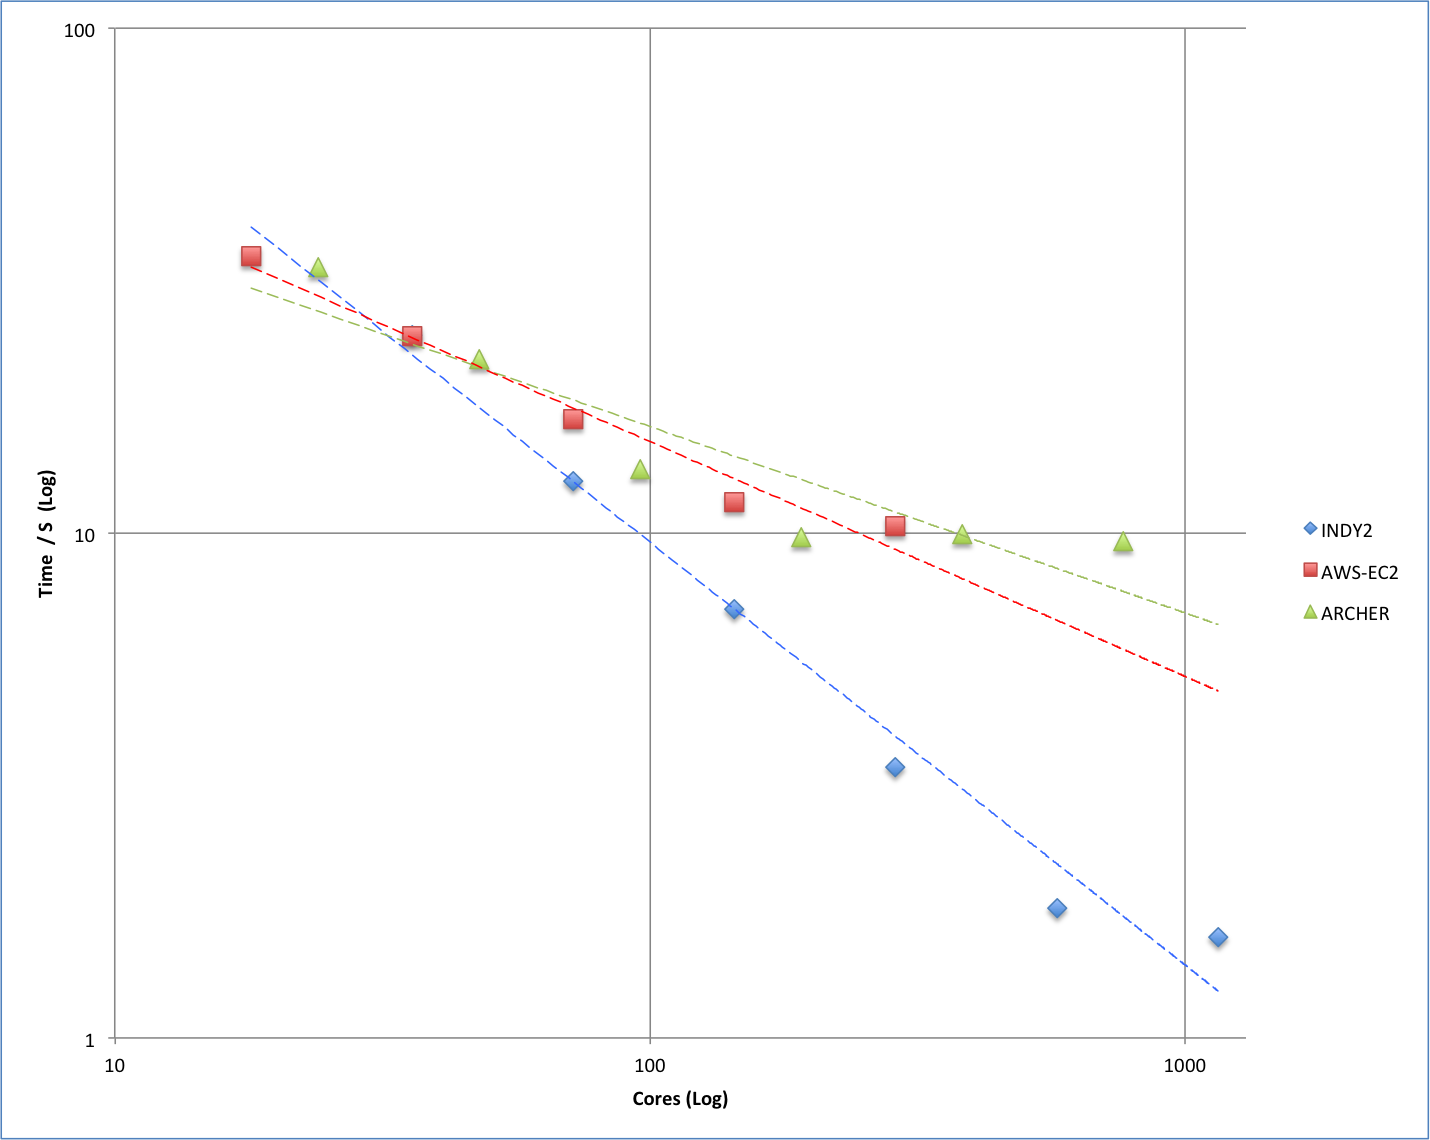
\includegraphics[keepaspectratio=true,scale=0.75]{../resources/evaluation/performance/overview.png}
 }
\captionof{figure}{HemeLB performance comparison} \label{fig:hemelb-perf-overview}%      only if needed  
\end{minipage}

\vspace{0.5cm}


In general, the performance of HemeLB with cloud infrastructure is worse when compared to ARCHER and INDY2. On each simulation instances with a different number of cores, we see slower simulation execution result when compared to the likes of the INDY2 machine and ARCHER supercomputer as observed on table \ref{table:perf}, \ref{table:perf-archer} and figure \ref{fig:hemelb-perf-overview}.

For the simulation, we use an input file which has 4,520,681 fluid sites\footnote{Available online at \url{https://github.com/SeiryuZ/HemeWeb/blob/master/deployment/roles/hemeweb_master/files/990_Example2-skeleton_corrected_tubed_smoothed.gmy}}  \footnote{Config for the simulation can be found online at \url{https://github.com/SeiryuZ/HemeWeb/blob/master/documents/resources/evaluation/performance/config.xml}}. According to the performance analysis by Groen et al. \citep{groen2013analysing}, HemeLB scales up near-linearly up to 32,768 cores. It also performs near its maximum efficiency when using 5,000 to 500,000 sites per core. This means that for the problem size we use, HemeLB should perform near maximum efficiency when using 9 cores up to 900 cores. Above that core counts, HemeLB simulation will incur a performance penalty.

The simulation time of INDY2 as observed in Figure \ref{fig:hemelb-perf-overview} follows this performance model accurately. It scales almost linearly up to 576 cores, and finally hit a performance degradation on 1152 cores. However, the result on AWS-EC2 shows that HemeLB hits performance degradation much early that it does not follow the performance models. The reason being is that the infrastructure has an underlying difference in the networking capabilities. AWS-EC2 offer 10 Gigabit per second interface \footnote{\url{https://aws.amazon.com/premiumsupport/knowledge-center/network-throughput-benchmark-linux-ec2/}} while dedicated HPC infrastructure often uses InfiniBand or Cray Aries router interconnectivity which provides higher throughput \cite{Quan:2014aa}. This result is in line with the benchmark that Mehrotra et al. did on NASA's HPC application \citep{mehrotra2012performance}. The performance degradation comes from the network and the virtualization overhead that this cloud platform has.  ARCHER supercomputer in this benchmark, however, shows the performance that does not follow the performance model closely. As we increase the core number, the simulation time decrease, but not near linearly. In addition, there is some dip in performance at 384 cores. This erratic results might be due to the random nature of the workload on ARCHER. 

ARCHER supercomputer has slower simulation time compared to INDY2, because of the difference of processors used in the compute node. ARCHER used a three-year-old 2.7 GHz, 12-core E5-2697 v2 Ivy Bridge processor. Compared to INDY2 which boasts the newer Broadwell-based Intel Xeon CPU E5-2695 v4 @ 2.10GHz. The number of thread inside those processors also differ, ARCHER has 24 while INDY2 has 36. This makes the performance difference. On the other hand for this evaluation, we use Amazon's c4.8xlarge EC2 instance which has Haswell-based E5-2666 v3 processor that has 36 virtual CPU cores. All these difference contributes toward the speed difference of the simulation results.

The scaling of the performance is where HemeWeb took a dive. It is apparent that with increased compute node, the network activity between the nodes become a bottleneck in the HemeWeb's case. The performance started to dip when we use 4 compute nodes which have 144 cores which perform worse than just using 1 compute node. However, the performance improves as we add more compute nodes. Roughly speaking, HemeWeb run HemeLB simulation in AWS-EC2 1.46 times slower and up to 11.27 times slower at its worst when compared to the INDY2's performance. The performance difference is more apparent when INDY2 scale really well with larger cores, while in AWS-EC2, it didn't.

\subsection{Price performance analysis}

To analyze the performance even further, we can compare the performance we get with the price we have to pay to run the infrastructure. In running the simulation for benchmark, we used c4.8xlarge linux instances on EU Ireland region which at the time of writing costs GBP 1.51\footnote{USD 1.96 converted to GBP on https://\url{www.oanda.com/currency/converter/} at 13th August 2016} per hour\footnote{\url{https://aws.amazon.com/ec2/pricing/}}. Phase 2 XC30 ARCHER supercomputer give access to screened project by compute hour which has the price of GBP 0.56 for research council which are partnered and GBP 1.33 for  non-partnered research council\footnote{Calculated on \url{http://archer.ac.uk/access/au-calculator/}}. INDY2 however have no public pricing released by the EPCC yet.

With these pricing information, we can deduce that using AWS EC2 is 2.69 times more expensive compared to using ARCHER with partnership and 1.13 times more expensive without partnership. With more costs, using HemeWeb has lower performance but comparable to the ARCHER supercomputer. This cost is also compounded with the fact that job will finish much slower when using HemeWeb on AWS-EC2 infrastructure. It potentially run 2.69 times more expensive per hour but 11.27 (CHANGE THIS WHEN NEW DATA ARRIVE) times much slower compared to using dedicated HPC infrastructure like ARCHER. If a job finish in 1 hour in INDY2, it can run for almost 12 hours (CHANGE THIS WHEN NEW DATA ARRIVE) on ARCHER at its worst, which will cost much more. However, because there are no price information yet on INDY2, we cannot make any price performance comparison between AWS-EC2 with INDY2 that has bigger performance gap. 


All of this performance pricing analysis however have to take into account of the model of business of the governing institution. On using Amazon's resources, one does not have to submit a proposal or go to a resource allocation community, he / she just need a credit cards and access will be given. In addition to that, Amazon employ the pay-as-you-go pricing scheme so it is very flexible in changing requirements or usage compared to ARCHER which allocate the resources at the start of the project. 


\section {Limitation of the evaluations}

\subsection{Usability evaluation}

When observing the evaluation, one might argue that 5 point scale used in the questionnaire is not enough as pointed out by Kraig Finstad \cite{finstad2010response}. In his research, he argued that 5 point scale for a questionnaire allows more room for respondents to interpolate their response. He compared the same version of usability study but with five-point and seven-point scale and found out that 3\% of the respondents answer to five point scale actually are interpolation, while the seven point scale have no interpolation. He concluded that administering usability study using seven point scale will achieve greater accuracy. However, I decided to use the five point scale of the questionnaire because of the limitation of google survey platform. 

\noindent%
\begin{minipage}{\linewidth}% to keep image and caption on one page
\makebox[\linewidth]{
  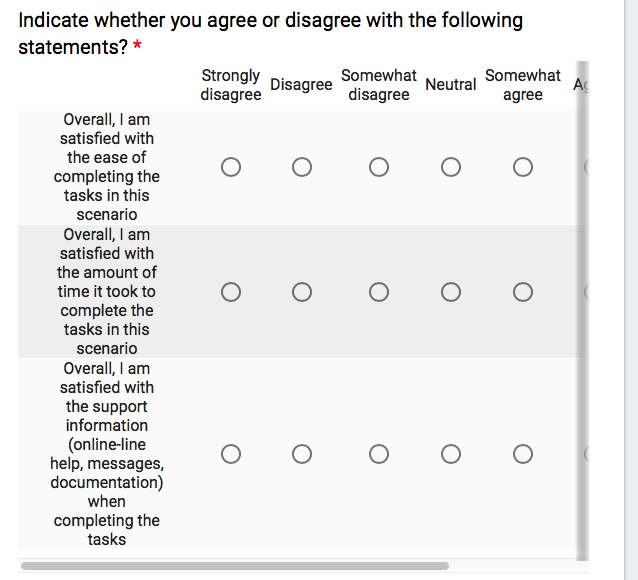
\includegraphics[keepaspectratio=true,scale=0.35]{../resources/images/google-limitation.png}
 }
\captionof{figure}{Google form hiding some options on 7 point scale} \label{fig:google-limit}%      only if needed  
\end{minipage}


\vspace{0.5cm}
\noindent%
\begin{minipage}{\linewidth}% to keep image and caption on one page
\makebox[\linewidth]{
  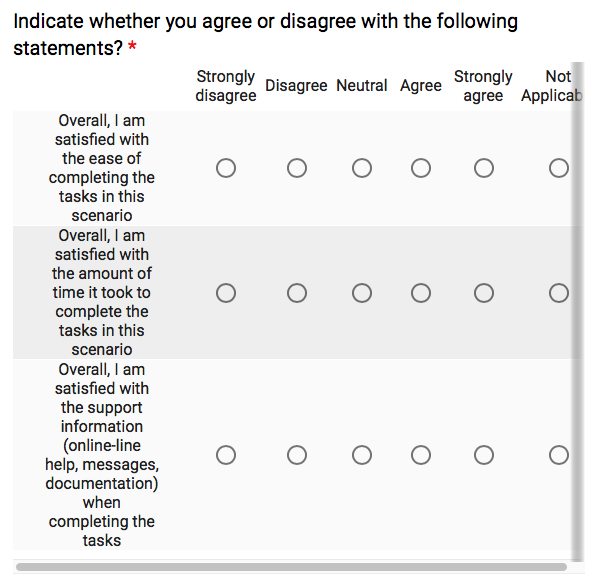
\includegraphics[keepaspectratio=true,scale=0.35]{../resources/images/google-limitation2.png}
 }
\captionof{figure}{Google form render 5 point scale rating better} \label{fig:google-limit2}%      only if needed  
\end{minipage}

\vspace{0.5cm}


Figure \ref{fig:google-limit} show the limitation of the platform. The response options are not rendered in complete, as in some are hidden in a scrolling element of the page. This leads to respondents have to scroll left and right to see the options and answers. I find this is a detriment to the respondents to do more work in answering the question so I decided to use 5 point scale to make sure everything is rendered better like shown in Figure \ref{fig:google-limit2}.


Another limitation of the study is the way the study compare the experience of doing the scenarios in the questionnaire between using web browser and using command line.  When measuring the usability of HemeWeb, respondents are asked to do the task in the web browser, compared to the task in command line where it is just described in an overview. This decision is made because we cannot make sure the respondents have the necessary tools to run or reproduce a simulation in their computers.  In addition, in order to run the scenario in command line interface, respondents have to install tools on their computer which are timely and prone to errors. I believe this will affect their sentiment in answering the survey questionnaire and decided against it.


\subsection{Performance evaluation}

On running the HemeLB simulation on the three systems compared, we cannot fully isolate the infrastructure from various system load the infrastructure is handling. The performance might be affected by other jobs running in the system, which is apparent in the case of ARCHER supercomputer where many jobs are executing at the same moment. The same case with INDY2. The performance benchmark might be not as accurate as a completely isolated environment, however it paints a pretty good picture of performance you get when using cloud vendors compared to the dedicated infrastructure. 

Also another limitation on the performance evaluation is that we cannot get more than 20 instances of c4.8xlarge instances on AWS. This causes the evaluation for AWS-EC2 cannot be done for the 1,152 cores to compare it directly with INDY2. Another limitation is that on ARCHER, it has 24 cores in 1 compute node compared to 36 in INDY2 and AWS-EC2. We wanted to measure the full load of the compute node, therefore we cannot get an exact apple to apple comparison. However, it could help in painting the general trend of the scaling capabilities and measure based on that.
 

% Activate the following line by filling in the right side. If for example the name of the root file is Main.tex, write
% "...root = Main.tex" if the chapter file is in the same directory, and "...root = ../Main.tex" if the chapter is in a subdirectory.
 
%!TEX root =  dissertation.tex

\chapter[Conclusion]{Conclusion}


% Activate the following line by filling in the right side. If for example the name of the root file is Main.tex, write
% "...root = Main.tex" if the chapter file is in the same directory, and "...root = ../Main.tex" if the chapter is in a subdirectory.
 
%!TEX root =  dissertation.tex

\chapter[Future work]{Future work}

To better support HemeLB simulation workflow, HemeWeb can be further improved. I suggest the following areas to be further developed in the future:

\begin{enumerate}
    \item Handle geometry generation step of HemeLB simulation workflow
    
    There are some steps which are not included in this project due to time constraints. One of them is the profile generation step. In this step, the domain experts should generate a profile file by pointing out how the simulation will run. They need to point where the blood will flow into the 3D  model of the vascular system, where it will flow out, the blood viscosity, and other various parameters that will affect the simulation result. This process will most likely require a graphical user interface for the domain experts to interact with.
    
    \item Viewing simulation result on the browser.
    
    HemeLB simulation outputs are  in a format that is viewable by a third party tool, ParaView. It will be ideal if HemeWeb can be one stop solution for HemeLB simulation that domain experts do not have to bother with all other tools to view the output of it. A ParaView integration can be done in the next step of the development so that simulation result can be directly viewed on the browser so users do not have to bother with an extra tool to configure and install.
    
    \item HemeLB simulation security
    
    As outlined in the implementation challenge of the project, security was not the main focus of this project. However, if this project is to be an essential part of the future medical decision, security will need to be addressed seriously. After all, the patient's private health information will be used for the simulation. A system using such highly private information should be better secured.

  Also, in line with the simulation security. HemeWeb instance should be better protected. Currently, HemeWeb does not have protected user area. Individuals without correct credentials can just run the simulation by entering the address of the application on their browser. This is not ideal because this simulation costs money. It should be better protected by having appropriate security measures against unauthorized access.

   \item HemeWeb notification

   Currently, users are asked to wait until simulation is done to get the output. The user had to keep the page open or checking back in an interval to see whether it is finished. It would be a better experience for users to be notified when a simulation is finished. The user can leave the web application and get back to it when notification is sent.


   \item Better interface to configure HemeLB parameters. 

      Echoing the suggestions that are collected during the evaluation of HemeWeb, there should be a better interface to configure HemeLB parameters. Currently, HemeWeb provides an online XML editor for users to update the HemeLB parameter directly. However, this process is prone to error and might not be the best interface for new users to configure HemeLB simulation. A better solution can be in the form of an automatic web form building from the XML file. With it, users can use the easier web form to select and specify the parameters for HemeLB simulation. This is currently not done because the active development cycle of HemeLB means that the format of XML is also actively developed and could create complications in the building in the form if the format is changed.
    
    \item Cloud vendor abstraction on web application
    
    One challenge of the project was the difference between cloud vendors. Due to the time constraint, the developed web application is tied down to amazon web services only. It would be ideal if HemeWeb could work on any cloud vendors with minimal changes. This is going to be more of a reconciling the difference between cloud vendors and make an abstraction layer that HemeWeb will need to call whenever it needs to interact with the cloud vendors' feature.
    
    The project did achieve cloud vendor abstraction for the deployment scripts. The infrastructure can be deployed to three different cloud vendors easily. They are google cloud platform, amazon web service, and digital ocean. However, the web application needs more work to achieve the similar feat. Infrastructure can be deployed on these infrastructures, but HemeWeb still cannot work on those infrastructure.
    
    To further improve the deployment, the abstraction layer should be able to handle deployment on dedicated HPC clusters. This will improve the flexibility of deployment even further that HemeWeb can be run not only on various cloud platforms, but also dedicated infrastructure that an institution built.
    
\end{enumerate}






%% Choose your favourite bibliography style here.
%\bibliographystyle{apalike}
\bibliographystyle{ieeetr}

%% If you want the bibliography single-spaced (which is allowed), uncomment
%% the next line.
% \singlespace

%% Specify the bibliography file. Default is thesis.bib.
\bibliography{thesis}



%% ... etc ...

%%%%%%%%
%% Any appendices should go here. The appendix files should look just like the
%% chapter files.
\appendix
% Activate the following line by filling in the right side. If for example the name of the root file is Main.tex, write
% "...root = Main.tex" if the chapter file is in the same directory, and "...root = ../Main.tex" if the chapter is in a subdirectory.
 
%!TEX root =  dissertation.tex
\chapter[Appendix: Dockerfile]{Appendix: Dockerfile}\label{app:dockerfile}



%%%%%%%%%%%%%%%%%%%%%%%%%%%%%%%%%%%%%%%%%%%%%%%%

\section{Cloud vendor specific provisioning scripts}

\lstinputlisting[caption=Stripped down version of the Dockerfile,label=lst:dockerfile]{../../hemelb_docker/Dockerfile}

% Activate the following line by filling in the right side. If for example the name of the root file is Main.tex, write
% "...root = Main.tex" if the chapter file is in the same directory, and "...root = ../Main.tex" if the chapter is in a subdirectory.
 
%!TEX root =  dissertation.tex
\chapter[Appendix: Deployment Script]{Appendix: Deployment Script}



%%%%%%%%%%%%%%%%%%%%%%%%%%%%%%%%%%%%%%%%%%%%%%%%

\section{Cloud vendor specific provisioning scripts}

\lstinputlisting[language=yaml, caption=Amazon web service specific provisioning script]{../../deployment/aws/provision.yml}

\lstinputlisting[language=yaml, caption=Digital ocean specific provisioning script]{../../deployment/digital_ocean/provision.yml}

\lstinputlisting[language=yaml, caption=Google cloud platform specific provisioning script]{../../deployment/google_cloud/provision.yml}



%%%%%%%%%%%%%%%%%%%%%%%%%%%%%%%%%%%%%%%%%%%%%%%%

\section{Cloud vendor specific deployment scripts}

\lstinputlisting[language=yaml, caption=Amazon web service specific deployment script]{../../deployment/aws/deploy.yml}

\lstinputlisting[language=yaml, caption=Digital ocean specific deployment script]{../../deployment/digital_ocean/deploy.yml}

\lstinputlisting[language=yaml, caption=Google cloud platform specific deployment script]{../../deployment/google_cloud/deploy.yml}






%%%%%%%%%%%%%%%%%%%%%%%%%%%%%%%%%%%%%%%%%%%%%%%%


\section{Common deployment script}

\lstinputlisting[language=yaml, caption=deploy.yml]{../../deployment/deploy.yml}



%%%%%%%%%%%%%%%%%%%%%%%%

\subsection{Common role}

\lstinputlisting[language=yaml, caption=roles/common/tasks/main.yml]{../../deployment/roles/common/tasks/main.yml}

\subsubsection{SSH specific common role}
\lstinputlisting[language=yaml, caption=roles/common/tasks/ssh.yml]{../../deployment/roles/common/tasks/ssh.yml}

\subsubsection{Package manager specific common role}
\lstinputlisting[language=yaml, caption=roles/common/tasks/apt.yml]{../../deployment/roles/common/tasks/apt.yml}


\subsubsection{Host specific common role}
\lstinputlisting[language=yaml, caption=roles/common/tasks/hosts.yml]{../../deployment/roles/common/tasks/hosts.yml}

\lstinputlisting[caption=roles/common/templates/hosts.j2]{../../deployment/roles/common/templates/hosts.j2}





%%%%%%%%%%%%%%%%%%%%%%%%
\subsection{Redis role}

\lstinputlisting[language=yaml, caption=roles/redis/tasks/main.yml]{../../deployment/roles/redis/tasks/main.yml}




%%%%%%%%%%%%%%%%%%%%%%%%

\subsection{Nginx role}

\lstinputlisting[language=yaml, caption=roles/nginx/tasks/main.yml]{../../deployment/roles/nginx/tasks/main.yml}


\lstinputlisting[caption=roles/nginx/templates/default.j2]{../../deployment/roles/nginx/templates/default.j2}

\lstinputlisting[caption=roles/nginx/templates/nginx.j2]{../../deployment/roles/nginx/templates/nginx.j2}




%%%%%%%%%%%%%%%%%%%%%%%%

\subsection{Postgresql role}
\lstinputlisting[language=yaml, caption=roles/postgresql/tasks/main.yml]{../../deployment/roles/postgresql/tasks/main.yml}

\lstinputlisting[caption=roles/postgresql/templates/pg\_hba.j2]{../../deployment/roles/postgresql/templates/pg_hba.j2}






% Activate the following line by filling in the right side. If for example the name of the root file is Main.tex, write
% "...root = Main.tex" if the chapter file is in the same directory, and "...root = ../Main.tex" if the chapter is in a subdirectory.
 
%!TEX root =  dissertation.tex

\chapter[Survey]{Survey}

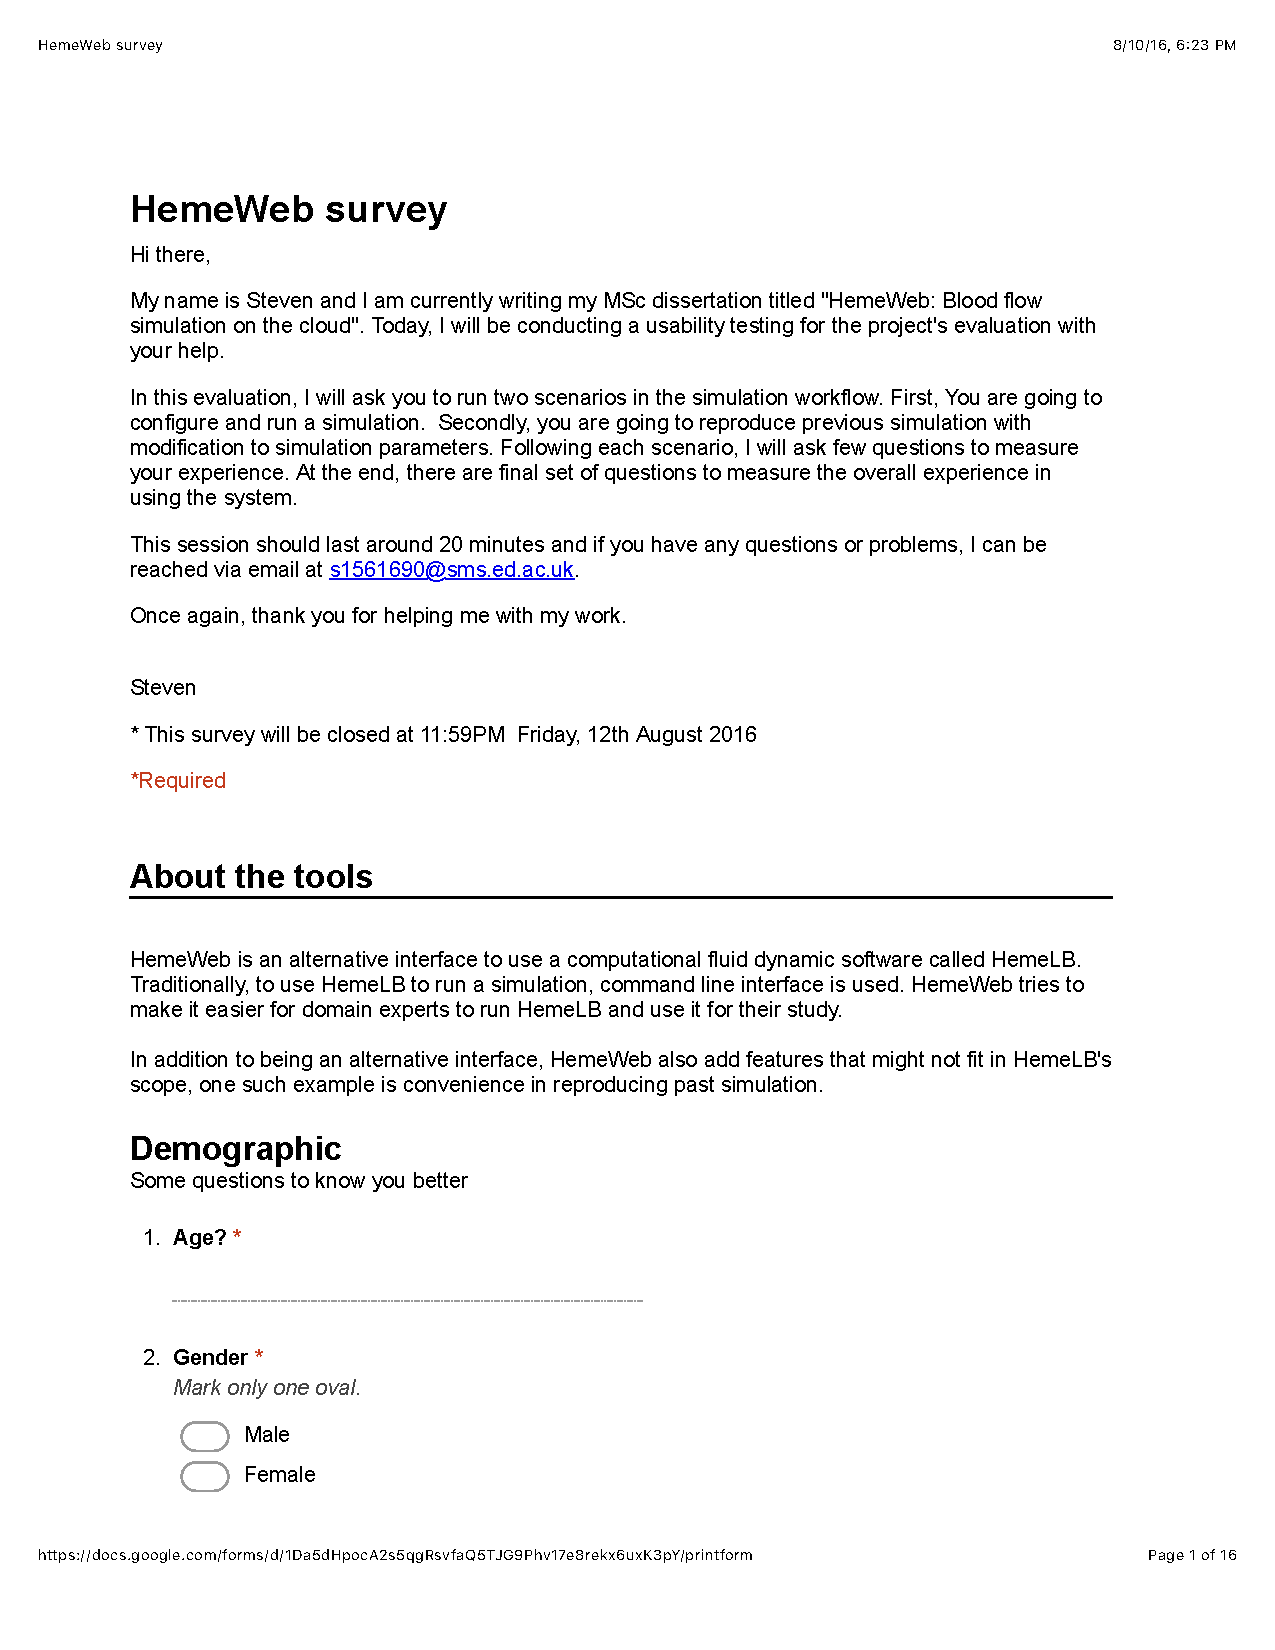
\includepdf[pages=-]{../resources/survey.pdf}


%% ... etc...

%% ... that's all, folks!
\end{document}
